\documentclass[a4paper, 11pt]{article}
\usepackage[text={15cm, 22cm}]{geometry}
\usepackage{fontspec}
\usepackage{newcomputermodern}
\usepackage[czech]{babel}
\usepackage[style=iso-numeric, backend=biber]{biblatex}
\addbibresource{citace.bib}

\usepackage{hyperref}
\hypersetup{
    colorlinks=true,
    citecolor=,
    linkcolor=,
    urlcolor=blue
}

\usepackage{minted}
\usepackage{float}
\floatstyle{ruled}
\floatname{listing}{Program}
\restylefloat{listing}

\floatstyle{plain} 
\newfloat{trace}{htbp}{lot}
\floatname{trace}{Výpis}

\usepackage{caption}
\captionsetup{font=small, labelfont=bf}
\captionsetup[listing]{labelsep=colon}

\usepackage{amsmath}

\usepackage{tikz}
\usetikzlibrary{shapes.geometric, arrows.meta, positioning}

\usepackage{microtype}
\usepackage{csquotes}
\usepackage[section]{placeins}

\usepackage{graphicx}
\makeatletter
\providecommand{\vcentcolon}{\mathrel{\mathchar"703A}}
\makeatother

\newcommand{\coloneqq}{%
  \mathrel{\mathop:\!\raisebox{0.2ex}{\scalebox{0.8}{$=$}}}
}

\usepackage{listings}
\definecolor{codegray}{rgb}{0.95,0.95,0.95}
\lstset{
    backgroundcolor=\color{codegray},
    basicstyle=\ttfamily\small,
    frame=single,
    rulecolor=\color{gray!30},
    breaklines=true,
    columns=fullflexible,
    keepspaces=true
}

\linespread{1.05}

\begin{document}

\begin{titlepage}
    \begin{center}
        {\Huge
            \textsc{Vysoké učení technické v~Brně}\\[0.5em]}
        {\huge
            \textsc{Fakulta informačních technologií}}\\
        \vspace{\stretch{0.382}}
        {\LARGE
            Statická analýza a verifikace -- projekt\\[0.8em]
            \textbf{CBMC -- C Bounded Model Checking}}\\[2em]
        \Large\today\\
        \vspace{\stretch{0.618}}
    \end{center}
    {\Large
    Bc. Ondřej Koumar\hfill\href{mailto:xkouma02@stud.fit.vutbr.cz}{xkouma02@stud.fit.vutbr.cz}}
\end{titlepage}

\section{Úvod}

CBMC je nástroj využívající techniky \emph{bounded model checking} pro verifikaci programů napsaných v~jazyce C.
Tato technika modeluje program pomocí \emph{bitově-vek\-to\-ro\-vé aritmetiky}, z~níž se poté generuje logická formule v~\emph{CNF} (konjunktivní normální formě).
Ta je potom předána \emph{SAT solveru}, který ověří její splnitelnost.
V~případě splnitelnosti existuje exekuční cesta v~programu s~konkrétním ohodnocením proměnných, která porušuje některou specifikovanou vlastnost.
Toto ohodnocení je pak protipříkladem k~původní hypotéze o~správnosti programu.

Nicméně nesplnitelnost formule neimplikuje, že je program korektní -- formálněji řečeno, je korektní do hloubky $k$, což je parametr určující hloubku rozbalení cyklu.
To také znamená, že pokud všechny cykly v~programu běží nejvíce $k$ iterací, pak nesplnitelnost formule dokazuje plnou korektnost programu vzhledem ke specifikacím.
Bounded model checking dokáže analyzovat pouze omezený počet iterací cyklů, a proto nemusí odhalit chyby, které se projeví až po větším počtu opakování.
Díky vysoké efektivitě SAT solverů je ale možné cyklus rozbalit na stovky iterací, a~proto se dá výsledek této formální verifikace považovat za \emph{dostatečně dobrý}.
Je ale zřejmé, že tato technika není dobře škálovatelná pro rozsáhlé projekty o~několika desítkách tisíc řádků kódu a~více.
Výsledná formule je totiž natolik velká, že SAT solver není schopen v~\emph{rozumném čase} tuto formuli vyřešit.

V~této technické zprávě se zaměřím na vnitřní architekturu CBMC, zejména na způsob překladu programu do \emph{SSA} (static single assignment) reprezentace, bit-vektorové modelování a~generování výsledné formule v~CNF.

\section{Technický popis nástroje}\label{sec:CBMC_Desc}

\subsection{Předzpracování programu}\label{sec:CBMC_Desc_Preprocessing}
Než je program převeden do SSA reprezentace, musí být provedeno předzpracování.
Architektura nástroje CBMC má několik vrstev a~je ukázána na obrázku~\ref{fig:cbmc_architecture}.
\begin{figure}[t]
    \centering
    \begin{tikzpicture}[
        % Styl bloku
        cbmc_block/.style={
                rectangle,
                draw=black,
                thick,
                text width=2.3cm,
                minimum height=1.2cm,
                align=center,
                font=\sffamily\footnotesize
            },
        % Styl sipky
        arrow/.style={
        -{Stealth[length=3mm]},
        thick
        },
        node distance=0.7cm and 0.7cm % svisle/vodorovne
        ]

        % Nodes
        \node (cmd) [cbmc_block] {Command Line\\Front End};

        \node (parser) [cbmc_block, below=of cmd] {C Parser};
        \node (type)   [cbmc_block, right=of parser] {Type Checking};
        \node (goto)   [cbmc_block, right=of type]   {GOTO Conversion};
        \node (static) [cbmc_block, right=of goto]   {Static Analysis \&\\Instrumentation};

        \node (symex)   [cbmc_block, below=1cm of parser] {Symbolic Execution};
        \node (cnf)     [cbmc_block, right=of symex] {CNF Conversion};
        \node (sat)     [cbmc_block, right=of cnf]   {SAT Solver};
        \node (counter) [cbmc_block, right=of sat]   {Counterexample\\Analysis};

        % Arrows
        \draw [arrow] (cmd) -- (parser);

        \draw [arrow] (parser) -- (type);
        \draw [arrow] (type) -- (goto);
        \draw [arrow] (goto) -- (static);

        \draw [arrow] (static.south) -- ++(0,-0.5cm) -| (symex.north);

        \draw [arrow] (symex) -- (cnf);
        \draw [arrow] (cnf) -- (sat);
        \draw [arrow] (sat) -- (counter);

    \end{tikzpicture}
    \caption{Architektura nástroje CBMC (převzato z~\cite{kroening2014cbmc})}
    \label{fig:cbmc_architecture}
\end{figure}
CBMC používá \emph{GOTO programy} jako přechodnou (\emph{intermediate}) reprezentaci.
V~tomto jazyce jsou všechny příkazy \texttt{switch}, \texttt{if}, cykly a~skoky převedeny na ekvivalentní \emph{guarded goto} příkazy.
Tento proces probíhá ve fázích \emph{GOTO conversion} a~\emph{Static Analysis \& Instrumentation} z~obrázku~\ref{fig:cbmc_architecture}.
Pro jednodušší formální popis je zde popsán převod zmíněných příkazů na guarded goto příkazy bez explicitního generování GOTO programu, nicméně CBMC tento mezikrok provádí.

\subsection{Rozbalení smyček}\label{sec:CBMC_Desc_LoopUnwinding}

Rozbalení probíhá následovně:
\begin{enumerate}
    \item Tělo cyklu je $k$-krát za sebou vnořeně zduplikováno.
    \item Řídící příkaz cyklu (\texttt{while}, \texttt{for}) je v~každé kopii nahrazen podmíněným příkazem \texttt{if}.
    \item Po rozbalení do hloubky $k$ je přidán \emph{unwinding assertion}.
\end{enumerate}

První dva kroky tohoto postupu jsou demonstrovány v~programu \ref{lst:loop_unwinding_nested} s~fixní hloubkou rozbalení $k = 2$.
\begin{listing}[t]
    \centering
    \setminted{fontsize=\small}

    \begin{minipage}[t]{0.45\textwidth}
        \textbf{Původní program}
        \vspace{0.3em}
        \begin{minted}[linenos, xleftmargin=1.6em]{c}
int i = 0;
int max = 0;

while (i < n) {
    if (data[i] > max) {
        max = data[i];
    }
    
    i++;
}
        \end{minted}
        \vspace{0.3em}
    \end{minipage}
    \hfill
    \vrule
    \hfill
    \begin{minipage}[t]{0.48\textwidth}
        \textbf{Rozbalený kód ($k=2$)}
        \vspace{0.3em}
        \begin{minted}[linenos, xleftmargin=1.6em, escapeinside=@@]{c}
int i = 0;
int max = 0;

if (i < n) {
    if (data[0] > max) 
        max = data[0];
    i++; 

    if (i < n) {
        if (data[1] > max) 
            max = data[1];
        i++; 
        assert(!(i < n)); @\label{line:unwinding_assertion}@
    }
}
        \end{minted}
        \vspace{0.3em}
    \end{minipage}
    \caption{Transformace cyklu \texttt{while} s neznámou horní mezí $n$ při fixní hloubce rozbalení $k=2$. }
    \label{lst:loop_unwinding_nested}
\end{listing}
Formálněji se loop rozbalení symčky dá zapsat následující rekurentní definicí.
Nechť $W = \texttt{while}(C)\{B\}$.
\[
    unwind(W, k) \coloneqq
    \begin{cases}
        \texttt{if}(C)\{B; \ unwind(W, k-1)\} & \text{pro } k > 0 \\
        \texttt{assert}(\neg C)               & \text{pro } k = 0
    \end{cases}
\]
Na řádku \ref{line:unwinding_assertion} v~rozbaleném kódu je již zmíněný unwinding assertion.
Tento assert slouží k~zaručení korektnosti verifikace.
Při převodu na SAT formuli tato podmínka říká, že cyklus byl rozbalen pro všechny iterace, které byly zapotřebí k~výpočtu.
Splnitelnost formule může odpovídat buď skutečnému porušení specifikace, nebo porušení unwinding assertion, které indikuje nedostatečnou hloubku rozbalení.
Intuitivně, pokud se verifikace \uv{nedostane} k~tomuto assertu, pak byly analyzovány všechny potřebné iterace cyklu a~analýza je korektní.

\subsection{Transformace programu do SSA a konstrukce rovnic}\label{sec:CBMC_Desc_SSATransformation}
Po předzpracování a~rozbalení cyklů se program skládá pouze z~podmíněných příkazů \texttt{if}, skoků vpřed a~assertů.
Tento kód je pak převeden na dvě bit-vektorové rovnice:
\begin{enumerate}
    \item $\mathcal{C}$ (constraints) -- množina omezení definující chování programu.
    \item $\mathcal{P}$ (properties) -- množina tvrzení, která musí platit.
\end{enumerate}

Proces převodu využívá formu \emph{SSA} (Static Single Assignment), kde je každá proměnná přiřazena nejvýše jednou.
Pokud se v~programu vyskytuje více zápisů do stejné proměnné $v$, je nutné rozlišit její jednotlivé verze v~čase ($v_1, v_2, \dots$).
Pro tyto účely je zavedena funkce přejmenování $\rho(e)$, kterou využívají všechny kroky převodu programu.
Tato funkce rekurzivně prochází výraz $e$ a~nahrazuje všechny výskyty proměnných jejich aktuálními verzemi platnými v~daném místě programu (např. $\rho(x + y) = x_1 + y_0$).


\subsubsection{Modelování řídícího toku -- guards}

Dalším krokem je převod dopředných skoků na ekvivalentní podmíněné příkazy \texttt{if}, ze kterých jsou posléze vygenerována přiřazení s~tzv. \emph{guardy}.
Ty reprezentují různé hodnoty, které by se mohly do proměnné přiřadit při předešlém větvení výpočtu.

\paragraph{Eliminace dopředných skoků.}
Cílem této fáze je odstranit příkaz \texttt{goto} tak, že kód, který se má přeskočit, je podmíněn negací podmínky skoku.
Ilustrativně, například
\begin{center}
    \begin{minted}{c}
        if (podminka) {
            goto label;
        }
        prikaz1;
        prikaz2;

        label:
            prikaz3;
    \end{minted}
\end{center}
je transformováno na ekvivalentní
\begin{center}
    \begin{minted}{c}
        if (!(podminka)) {
            prikaz1;
            prikaz2;
        }
        prikaz3;        
    \end{minted}
\end{center}
Algoritmus pracuje následovně.
Uvažujme program $P$ jako sekvenci příkazů.
Nechť $I$ je příkaz skoku \texttt{goto} $l$, kde $l$ je návěští definované v~programu za příkazem $I$.
Program za příkazem skoku (označme jej např. jako $P_{rest})$ je rozdělen na tři části vzhledem k~návěští~$l$:
\[
    P_{rest} = \underbrace{\text{blok } X}_{\text{kód k přeskočení}} l: \underbrace{\text{blok } Y}_{\text{zbytek programu}}
\]
Samotný příkaz \texttt{goto $l$} je odstraněn.
Nechť $g$ je aktuální podmínka, pod kterou se má blok $X$ vykonat.
Aby byla zachována sémantika původního skoku, blok $X$ se provede právě tehdy, když se skok neprovedl.
Příkazy bloku $X$ jsou tedy obaleny podmínkou $\neg g$:
\begin{center}
    \texttt{if ($\neg g$) \{ \textrm{blok }$X$ \} \textrm{blok }$Y$}
\end{center}
Protože program před touto transformací už je zpracován a~obsahuje pouze \texttt{if} příkazy, $g$ může být komplexní formule obsahující libovolný počet omezení (v~praxi to ale bude nanejvýš do několika desítek).
Formálně, nechť $e_1,\ldots,e_n$ jsou výrazy, které jsou podmínkami, aby se běh programu dostal k~aktuálně zpracovávanému skoku \texttt{goto $l$}.
Potom:
\[
    g \coloneqq
    \begin{cases}
        \bigwedge\limits_{i=1}^{n} e_i & \text{pro } n \geq 1 \\
        true                           & \text{jinak}
    \end{cases}
\]

Tímto procesem se tok řízený skoky převede na tok strukturovaný podmínkami \texttt{if}, což je nezbytné pro další krok, kde se podmínky stanou součástí definic proměnných. \cite{clarke2003hardware}

\subsubsection{Eliminace ukazatelů}
Ještě před generováním SSA rovnic a přejmenováním proměnných provádí CBMC eliminaci všech operací dereference ukazatelů.
To je nutné kvůli tomu, že výsledná rovnice v~bit-vektorové logice nepracuje s~konceptem paměťových adres, ale jednotlivými proměnnými.

Tento proces je realizován \emph{dereferenční funkcí} $\phi(e, g, o)$, jejímž vstupem je výraz~$e$ (ukazatel), aktuálně platný guard~$g$ a~offset~$o$.
Tato funkce transformuje výraz s~dereferencí na výraz bez ní, a~to tak, že si ke každému ukazateli drží tzv. \emph{points-to} množinu, ve které jsou všichni potenciální kandidáti, na které může daný ukazatel ukazovat.
Pro každého z~těchto kandidátů se vygeneruje identická sada omezení.
Když SAT solver postupně řeší výslednou formuli, dosazování do těchto omezení si můžeme představit jako \uv{výběr} správného kandidáta.
Tento přístup je nadaproximace řešení, což znamená, že nástroj je konzervativní a~může vygenerovat formuli, která je splnitelná, ale není reálné, aby takový případ nastal (\emph{false positive}).

V~jazyce C jsou dostupné dva typy dereference, a~to operátor dereference $*$ a~operátor indexování polí $[]$.
Funkce $\phi$ pracuje pro oba operátory stejným způsobem, jen jsou jinak manipulovány offsety.
Výraz $*e$ si můžeme představit jako $e[0]$; offset pro operátor $*$ je tedy vždy 0, zatímco pro indexaci pole je to obecně $o$.
\[
    *e \longrightarrow \phi(e, g, 0) \qquad e[o] \longrightarrow \phi(e, g, o)
\]

Funkce $\phi$ je definována podle toho, jakého typu je výraz $e$.
\begin{enumerate}
    \item \textbf{Ukazatel}: Nechť $p$ je takový ukazatel.
          Dosud vygenerovaná rovnice nebo guard $g$ musí obsahovat rovnost $\rho(p) = e'$, kde $e'$ je výraz.
          Ukazatel $p$ je derefencován aplikací $\phi$ na $e'$.
          \[
              \phi(p, g, o) \coloneqq \phi(e', g, o)
          \]

    \item \textbf{Pole}: Nechť $a$ je takové pole.
          Symbol $e$ je pouze aliasem pro $\&a[0]$.

    \item \textbf{Adresa jiného symbolu}: Tedy ekvivalent k~$e = \&s$.
          V~tomto případě je hodnota $\phi(e, g, o)$ rovna pouze symbolu $s$, protože dereference adresy symbolu je právě ten symbol.
          Hodnota offsetu $o$ v~tomto případě musí být 0.
          Navíc je provedena typová kontrola.
          \[
              \phi(\&s, g, o) \coloneqq s
          \]

    \item \textbf{Adresa prvku pole}: Tedy $e = \&a[i]$ pro nějaké pole $a$ a~pozici $i$.
          Dereference adresy prvku pole $\&a[i]$ je právě ten prvek $a[i]$.
          Stejně jako v~předchozím případě je provedena typová kontrola pro prvky pole.
          \[
              \phi(\&a[i], g, o) \coloneqq a[i + o]
          \]

    \item \textbf{Podmíněný příkaz (ternární operátor)}: V~takovém případě je funkce $\phi$ aplikována rekurzivně pro oba případy a~podmínka $c$ je přidána do guardu.
          \[
              \phi(c \; ? \; e' : e'', g, o) \coloneqq c \; ? \; \phi(e', g \land c, o) : \phi(e'', g \land \neg c, o)
          \]

    \item \textbf{Výraz s ukazatelovou aritmetikou}: Výraz, kde se sčítá ukazatel s~nějakým celým číslem.
          Předpokládejme, že $e'$ je ukazatel a~$i$ je celé číslo.
          Protože $i$ je pouze offset v~paměti, je tato hodnota přičtena k~offsetu $o$ a~funkce $\phi$ je rekurzivně volána pro výraz $e'$.
          Opět je provedena typová kontrola formou \texttt{assert}u.
          \[
              \phi(e' + i, g, o) \coloneqq \phi(e', g, o + i)
          \]

    \item \textbf{Přetypování ukazatelů}: Výraz typu $(T*)e'$, kde $T$ je nějaký typ.
          Funkce $\phi$ je aplikována na výraz $e'$, typové kontroly jsou pokryty v~ostatních případech, tudíž není třeba žádnou další přidávat.
          \[
              \phi((T*)e', g, o) \coloneqq \phi(e', g, o)
          \]

    \item \textbf{Jiný typ výrazu}: Dle autorů v~\cite{clarke2003behavioral} pro jiné výrazy (v~ANSI-C, pro které je tento nástroj implementován) není definována sémantika, a~proto nástroj do množiny omezení (bude popsáno v~následující sekci) přidává \texttt{assert}, že se sem kód nesmí dostat (tedy \texttt{assert($\neg g$)}).
\end{enumerate}

Situaci lze demonstrovat na jednoduchém příkladu.
Mějme ukazatel $p$, který byl někde před aktuálním bodem v~programu definován a~nástroj zjistil, že může ukazovat na proměnné $\{v_1, v_2, \dots, v_n\}$.
Tato množina je právě zmiňovanou \emph{points-to} množinou.
Pro zjednodušení řekněme, že proměnné $v_1, \dots, v_n$ jsou primitivního datového typu.
Funkce $\phi$ s~\emph{points-to} množinami pracuje následovně.

Nástroj narazí na výraz $*p$.
Pokud je tento výraz na pravé straně, máme jednodušší případ.
Stačí si pouze ověřit, na kterou proměnnou vlastně aktuálně ukazatel ukazuje a~dle toho vybrat správnou hodnotu.
Tím pádem bude hodnota funkce $\phi$ podmíněným výrazem, kde se budou brát v~potaz všechny možnosti proměnných z~\emph{points-to} množiny.
\[
    \phi(*p,g,0) \coloneqq (p == \&v_1​) \; ? \; v_1 ​: ((p == \&v_2 ) \; ? \; v_2 : (\dots))
\]

\noindent Pokud je ukazatel použit na levé straně přiřazení (např. $*p = x$), nástroj to vyřeší podobným způsobem, protože přesně neví, kterou hodnotu aktualizovat.
Nejjednodušší způsob je toto přiřazení vyřešit rozkladem na podmíněné příkazy pro všechny kandidáty z~\emph{points-to} množiny.
Původní přiřazení $*p = x$ je tedy nahrazeno sekvencí:
\begin{align*}
     & \texttt{if } \texttt{(}p == \&v_1\texttt{) } \texttt{\{}\ v_1 = x;\ \texttt{\}}      \\
     & \texttt{else if } \texttt{(}p == \&v_2\texttt{) } \texttt{\{}\ v_2 = x;\ \texttt{\}} \\
     & \dots
\end{align*}
Každá z~těchto větví je následně zpracována standardním způsobem, jako bylo uvedeno na začátku této sekce, tedy rekurzivní aplikací funkce $\phi$ na jednotlivé příkazy.

\subsubsection{Generování omezení a vlastností}
Po normalizaci řídícího toku a~analýze ukazatelů je možné generovat rovnice zmíněné na začátku této kapitoly, $\mathcal{C}$ a~$\mathcal{P}$.
Tento proces se provádí pomocí stejnojmenných funkcí $\mathcal{C}(p, g)$ a~$\mathcal{P}(p, g)$.
Obě dvě jsou definovány dle aktuálního $p$.

Pokud $p$ je podmíněný příkaz s~podmínkou $c$, \texttt{then}-blokem $I$ a~\texttt{else}-blokem $I'$, pak obě dvě funkce jsou rekurzivně aplikovány pro oba dva bloky.
Pro $I$, $\rho(c)$ je přidáno do guardu, pro $I'$ je přidáno $\neg \rho(c)$.
Výsledky zanoření rekurze jsou pak spojeny konjunkcí.
\begin{align*}
    \mathcal{C}(\texttt{if (c) } I \texttt{ else } I', g) & \coloneqq \mathcal{C}(I, g \land \rho(c)) \land \mathcal{C}(I', g \land \neg \rho(c)) \\
    \mathcal{P}(\texttt{if (c) } I \texttt{ else } I', g) & \coloneqq \mathcal{P}(I, g \land \rho(c)) \land \mathcal{P}(I', g \land \neg \rho(c))
\end{align*}

Pro sekvenci příkazů jsou funkce také definovány rekurzivně.
Nechť $p$ je sekvence příkazů složená z~$I$ a~$I'$.
Potom jsou obě funkce rekurzivně aplikovány na $I$ a~$I'$ následujícím způsobem:
\begin{align*}
    \mathcal{C}(I;\;I', g) & \coloneqq \mathcal{C}(I, g) \land \mathcal{C}(I', g) \\
    \mathcal{P}(I;\;I', g) & \coloneqq \mathcal{C}(I, g) \land \mathcal{P}(I', g)
\end{align*}

Nechť $p$ je tvrzení (\emph{assertion}) s~argumentem $a$.
Tento argument je přejmenován funkcí $\rho$  a~vrácen jako vlastnost programu, která se bude ověřovat.
Střežen je guardem $g$.
Funkce $\mathcal{C}$ s~tvrzeními nedělá nic, respektive přidá $true$ do konjunkce.
\[
    \mathcal{P}(\texttt{assert(}a\texttt{)}, g) \coloneqq g \implies \rho(a)
\]

Přiřazení jsou také přidávána jako omezení do $C$ po přejmenování proměnných.
Pokud proměnná $v$ má být přepsána hodnotou nového výrazu $e$ pod guardem $g$, pak pokud $g$ platí, proměnná je přepsána novým výrazem a~pokud ne, proměnná si zachovává stejnou hodnotu.
Tento problém je řešen \uv{ternárním operátorem}, který bere ohled na daný guard.
\[
    \mathcal{C}(v = e, g) \coloneqq v_\alpha = g \; ? \; \rho(e) : v_{\alpha-1}
\]
Intuitivně, guard $g$ nemůže být vyhodnocen během transformace, tudíž musí být součástí tohoto omezení.

Pro pole hodnot je konstrukce těchto omezení komplikovanější.
Mějme příkaz $v[a] = e$.
Hodnota v~poli $v_\alpha$ na indexu $i$ je rovno $\rho(e)$ pokud guard $g$ platí a~$i = a$, jinak $v_{\alpha}[i] = v_{\alpha - 1}[i]$.
Pole jsou modelována $\lambda$-funkcemi:
\[
    \mathcal{C}(v = e, g) \coloneqq v_\alpha = \lambda i: (g \land i = \rho(a))\; ? \; \rho(e) : v_{\alpha - 1}[i]
\]
Intuitivně vysvětleno, pole je funkce, která pro daný index $i$ vrátí $\rho(e)$, tedy novou hodnotu přepsanou výrazem $e$, pokud $i = \rho(a)$ (a samozřejmě musí platit guard $g$), jinak vrací hodnotu ze starého pole $v_{\alpha-1}[i]$.
Do formule s~tvrzeními musí být přidána kontrola mezí pole.
\[
    \mathcal{P}(v = e, g) \coloneqq 0 \leq \rho(a) \land \rho(a) < len(v_\alpha)
\]

Dalším problémem jsou strukturované datové typy.
Autoři v~\cite{kroening2016decision} zmiňují, že struktury jsou v~podstatě \emph{syntactic sugar} pro pole.
Nicméně během analýzy známe velikost struktury a~offsety jednotlivých položek struktury.
Proto není třeba reprezentovat struktury pomocí $\lambda$-funkce, ale můžeme do nich přistupovat statickým indexem, respektive odkazy na jednotlivé členy.
Nechť $s$ je proměnná typu \texttt{struct} a~příkaz přiřazení je $s.f = e$, kde $f$ je člen této struktury.
Potom nová verze struktury $s_\alpha$ je pro každý člen $m$ definována následovně:
\[
    \mathcal{C}(s.f = e, g) :=
    \begin{cases}
        g \; ? \; \rho(e) : s_{\alpha - 1}.f & \text{ pro } m = f    \\
        s_{\alpha - 1}.m                     & \text{ pro } m \neq f
    \end{cases}
\]

\subsection{Bit-vektorová aritmetika}\label{sec:CBMC_Desc_BitVectorArithmetics}

V~předchozí kapitole byly definovány rovnice omezení a~vlastností ($\mathcal{C}$ a~$\mathcal{P}$) nad proměnnými programu.
Tyto proměnné jsou běžně chápány jako proměnné s~neomezenou doménou; to ale neplatí v~hardwaru.
Každá proměnná v~jazyce C má pevnou bitovou šířku, protože jazyk C je nízkoúrovňový jazyk, který se překládá do strojového kódu a~tím pádem musí respektovat architekturu, na které je zdrojový kód přeložen.
Všechny proměnné jsou tedy reprezentovány jako \emph{bitové vektory} pevné šířky $w$.
Díky této reprezentaci může nástroj hledat chyby související s~bitovou aritmetikou, jako jsou například \emph{přetečení}, \emph{podtečení}, chyby spojené s~reprezentací čísel\dots
Všechny operace se dají zapsat jako operace nad množinami zbytků po dělení $2^w$, jedná se tedy o modulární aritmetiku (při použití vhodné reprezentace, např. dvojkový doplněk).
Například sčítání:
\[
    a +_w b = (a + b) \pmod{2^w}
\]

CBMC tohoto faktu využívá a~pro zdrojový program staví jeho reprezentaci ve formě ekvivalentního elektrického obvodu, který provádí primitivní operace (sčítání, apod.).
CBMC řeší otázku \uv{Existuje nastavení vstupních bitů tak, aby výstup byl '1'?} (tedy existuje ohodnocení proměnných tak, že $\mathcal{C} \land \neg \mathcal{P}$?).
Proto daný obvod musí převést na logickou formuli, kterou potom předá SAT solveru.

\subsubsection{Konstrukce obvodů (Flattening)}
Každá bit-vektorová proměnná $x$ o~šířce $w$ je rozložena na vektor $w$ výrokových proměnných $x_0, \dots, x_{w-1}$.
Aritmetické a~relační operátory jsou následně nahrazeny ekvivalentními hardwarovými obvody.

Jako příklad uvažujme sčítání $s = a + b$.
CBMC pro tuto operaci vygeneruje logický obvod odpovídající tzv.~\emph{Ripple Carry Adder}.
Tento obvod se skládá z~kaskády úplných sčítaček.
Pro každý bit $i$ jsou vygenerovány výrokové formule definující výsledný bit $s_i$ a~přenos do vyššího řádu $c_{i+1}$:
\begin{align*}
    s_i     & \iff a_i \oplus b_i \oplus c_i                         \\
    c_{i+1} & \iff (a_i \land b_i) \lor (c_i \land (a_i \oplus b_i))
\end{align*}
Kde $\oplus$ značí operaci XOR.
Obdobně jsou konstruovány obvody pro odčítání, porovnávání (sčítačky, negace), bitové posuny (multiplexory), násobení, apod.
Tato technická zpráva ilustruje techniku flatteningu na jednoduchém příkladu sčítání; její podrobný popis je uveden v~\cite[kap.~6.2]{kroening2016decision}.

\subsubsection{Převod do CNF}
Výsledek konstrukce obvodu je orientovaný acyklický graf reprezentující ten daný zkonstruovaný obvod.
Vrcholy tohoto grafu jsou logická hradla, hrany mezi nimi jsou dráty mezi hradly.
Tento graf reprezentuje formuli:
\[
    \Phi = \mathcal{C} \land \neg \mathcal{P}
\]
Pro použití moderních SAT solverů je nutné převést tento graf do \emph{konjunktivní normální formy} (CNF).
Přímý převod by mohl vést k~exponenciálnímu nárůstu velikosti formule, proto se využívá \emph{Tseitinova transformace} \cite{tseitin1983complexity}.
To je transformace původní formule $\varphi$ na \emph{ekvisplnitelnou} formuli $\psi$, což znamená, že $\varphi$ je splnitelná právě tehdy, když $\psi$ je splnitelná.
Jinými slovy, existuje model formule $\varphi$ právě tehdy, když existuje model formule $\psi$.
Tyto modely ale mohou být libovolné a~nemusí pro obě formule existovat stejný počet modelů, aby byla zachována ekvisplnitelnost.

\paragraph{Tseitinova transformace.}
Pro lepší intuici uvažujme jednoduchý logický obvod reprezentující výraz $z = (a \land b) \lor c$.
Jak bylo zmíněno, algebraické převody přes distributivní zákony nejsou proveditelné.
Tseitinova transformace místo toho zavádí pomocnou proměnnou pro každý mezivýsledek (výstup hradla).

Nechť $w_1$ je pomocná proměnná reprezentující výstup hradla AND ($a \land b$).
Původní výraz se tím rozpadne na dvě jednoduché rovnice (lokální omezení):
\begin{align*}
    w_1 & \iff (a \land b)  \\
    z   & \iff (w_1 \lor c)
\end{align*}
Každá z~těchto ekvivalencí je poté standardním algebraickým převodem převedena na sadu klauzulí:
\begin{align*}
    w_1 \iff (a \land b) & \equiv (w_1 \implies (a \land b)) \land ((a \land b) \implies w_1)                   \\
                         & \equiv (\neg w_1 \lor (a \land b)) \land (\neg(a \land b) \lor w_1)                  \\
                         & \equiv (\neg w_1 \lor a) \land (\neg w_1 \lor b) \land (\neg a \lor \neg b \lor w_1)
\end{align*}
Stejným způsobem se zpracuje výraz $z \iff (w_1 \lor c)$, kde $w_1$ reprezentuje výsledek konjunkce v~původním výrazu $z = (a \land b) \lor c$.
\[
    z \iff (w_1 \lor c) \equiv (\neg w_1 \lor z) \land (\neg c \lor z) \land (w_1 \lor c \lor \neg z)
\]
Výsledná SAT formule je konjunkcí všech šesti klauzulí.
Protože klauzule pro konkrétní typy hradel jsou vždy stejné, nemusíme složitě algebraicky počítat převody ekvivalencí do CNF.
Místo toho můžeme mít například tabulky, kde pro konkrétní hradlo najdeme výraz v~CNF, který můžeme do výsledné formule přidat.
Výhoda Tseitinovy transformace je maximálně lineární nárůst délky formule.

Formule je následně předána SAT solveru.
Pokud solver nalezne splnitelné ohodnocení (SAT), znamená to, že existuje kombinace vstupních bitů, která vede k~porušení vlastnosti~$\mathcal{P}$ a~z~modelu solveru je rekonstruován protipříklad.
V opačném případě (UNSAT) je program (do hloubky $k$) korektní.

\section{Demonstrace základních vlastností CBMC}\label{sec:CBMC_Demo}

V~této sekci se budeme věnovat experimentům, které demonstrují schopnosti i~limity nástroje CBMC.
Nejprve představíme sadu jednoduchých, cíleně zvolených příkladů, jejichž cílem je ilustrovat, jak CBMC detekuje různé typy chyb (přetečení, chyby práce s~pamětí, apod.) a~jakým způsobem prezentuje nalezené protipříklady.

Druhá část sekce je věnována řadícímu algoritmu Merge sort.
Tento algoritmus je výrazně komplexnější než úvodní příklady, protože využívá rekurzi a~dynamickou práci s~poli.
Na této úloze demonstrujeme použitelnost nástroje CBMC na složitějším algoritmu a~diskutujeme jeho omezení, která vyplývají z~techniky bounded model checkingu.

\subsection{Demonstrace funkcionality na syntetických příkladech}\label{sec:CBMC_Demo_Synthetic}

V~\href{https://github.com/diffblue/cbmc}{repozitáři} autorů nástroje CBMC je rozsáhlá sada jednoduchých testů, které slouží především k~regresivnímu testování nástroje.
Tyto příklady jsou ale záměrně velmi minimalistické a~jejich podstatou není ilustrovat chování nástroje na realističtějších programech.
Proto jsem se nakonec rozhodl napsat si několik jednoduchých kódů v~jazyce C, z~nichž každý má přibližně 20~řádků.
Každý z~těchto příkladů je navržen tak, aby demonstroval určitou vlastnost nebo slabinu CBMC na stále jednoduchém, ale srozumitelném kódu, pro který se dá vysvětlit jeho praktické využití.

\subsubsection{Příklad 1 -- Sekvence podmínek vedoucí k porušení vlastnosti}

Cílem tohoto příkladu je demonstrovat jednu z~hlavních sil model checkingu kombinovaného se SAT solvingem, konkrétně schopnost automaticky nalézt takovou kombinaci vstupních hodnot, která vede k~porušení sledované vlastnosti programu, a~to i~v~přítomnosti složitě zanořených podmínek.
Kód v~programu \ref{lst:complex_condition} obsahuje jednoduchou funkci, kde po sekvenci podmínek je z~funkce vrácena hodnota $-1$, která reprezentuje chybu.
Funkce \texttt{nondet\_int()} reprezentuje nedeterministické hodnoty, například vstupy od uživatele do programu.
\begin{listing}[h]
    \caption{Porušení \texttt{assert}u po splnění několika komplexních podmínek.}
    \label{lst:complex_condition}
    \begin{minted}[linenos, xleftmargin=1.6em, escapeinside=@@]{c}
#include <assert.h>

int nondet_int();
int complex_condition(int a, int b)
{
    if (a > 1000 && b > 1000) {
        if (a == b + 53) {
            if ((a % 2 == 0) && (b % 2 != 0)) {
                return -1;
            }
        }
    }
    return 0;
}

int main()
{
    int x = nondet_int();
    int y = nondet_int();
    int result = complex_condition(x, y); @\label{line:complex_condition}@
    assert(result != -1);
    return 0;
}  
    \end{minted}
\end{listing}

Ačkoliv je uvedený příklad uměle zjednodušený, obdobné situace se mohou vyskytovat i~v~reálných programech.
Takové podmínky pravděpodobně nebudou hned za sebou v~jedné funkci, mohou být stovky řádků kódu od sebe.
Splnění určité kombinace podmínek může vést například k~neoprávněnému zvýšení práv (může vést na útok \emph{privilege escalation}).
SAT solver najde přesné ohodnocení proměnných \texttt{a} a~\texttt{b}, které poruší \texttt{assert} na řádku~\ref{line:complex_condition}.

CBMC po spuštění s~tímto zdrojovým programem vygeneruje očekávaný výstup:
\begin{lstlisting}
[main.assertion.1] line  assertion result != -1: FAILURE
\end{lstlisting}

\noindent Tato chyba ovšem není jediná v~uvedeném zdrojovém kódu.
Může totiž dojít k~přetečení při sčítání operandů \texttt{b} a~53 ve funkci \texttt{complex\_condition(int a, int b)}, výsledek tedy může být chybný.
Této problematice se budeme věnovat v~následujícím příkladu.

\subsubsection{Příklad 2 -- přetečení výsledku operace}

Celočíselné přetečení demonstrujeme na kódu, který je typický například pro implementaci binárního vyhledávání v~řazeném poli.
Jedná se o~výpočet středu celočíselného intervalu\footnote{Tento pojem není technicky zcela přesný; pro účely tohoto textu však budeme celočíselný interval chápat jako množinu $\{l, l+1, \dots, h\}$.}.

\begin{listing}[ht]
    \caption{Chybný výpočet hodnoty poloviny intervalu $\langle l, h \rangle$.}
    \label{lst:incorrect_mid_point}
    \begin{minted}[linenos, xleftmargin=1.6em, escapeinside=||]{c}
int nondet_int();
int main()
{
    int l = nondet_int();
    int h = nondet_int();
    int m = (l + h) / 2;
    return 0;
}
    \end{minted}
\end{listing}

\noindent CBMC při analýze programu detekuje přetečení při sčítání proměnných \texttt{l} a~\texttt{h}:
\begin{lstlisting}
[main.overflow.1] line 6 arithmetic overflow on signed + in l + h: FAILURE
\end{lstlisting}
Tato chyba je velmi zrádná, protože běžné testování ji často vůbec neodhalí.
Při použití menších datových typů pro indexy polí se může projevit již během testování, avšak pro 32bitová celá čísla se s~vysokou pravděpodobností objeví až po nasazení.
Chybu lze odstranit záměnou $\frac{l+h}{2}$ za $l + \frac{h-l}{2}$ (je ale třeba zaručit $h \geq l$).
V~druhém případě se při výpočtu středu nedostaneme mimo interval $\langle l, h \rangle$ při výpočtu.

\subsubsection{Příklad 3 -- přístup mimo meze pole}

Tento příklad demonstruje přístup mimo meze pole způsobený nedostatečnou kontrolou iterační proměnné.
Podobná situace může v~praxi vzniknout například při práci s~daty, jejichž velikost je získána z~externího zdroje (uživatelský vstup, soubor, síťová komunikace,\dots) a~její hodnota není dostatečně ověřena.

\begin{listing}[t]
    \caption{Zápis mimo meze pole způsobený neověřenou hodnotou proměnné \texttt{n}.}
    \label{lst:out_of_bounds}
    \begin{minted}[linenos, xleftmargin=1.6em]{c}
int nondet_int();

int main()
{
    int arr[5];

    for (int i = 0; i < 5; i++) {
        arr[i] = nondet_int();
    }

    int n = nondet_int();
    if (n > 0) {
        for (int i = 0; i < n; i++) {
            arr[i] = 0;
        }
    }

    return 0;
}
    \end{minted}
\end{listing}

\noindent V~uvedeném kódu v~programu \ref{lst:out_of_bounds} není hodnota proměnné \texttt{n} nijak omezena shora.
Pokud \texttt{n} bude mít hodnotu větší než velikost pole \texttt{arr}, dojde k~zápisu mimo jeho meze, což je v~jazyce C nedefinované (pro dynamicky alokované pole často vede k~chybě přístupu do paměti, např. \emph{segmentation fault}).

V~reálných programech se chyba může vyskytnout například při mazání částí polí nebo zpracování pouze části vstupních dat, kdy se implicitně předpokládá, že vstupní hodnota nepřekročí velikost alokovaného úložiště.
Tato chyba je lépe testovatelná než přetečení celočíselných operandů, nicméně testování mezních hodnot může být lehce přehlédnuto.
CBMC je schopen tuto chybu detekovat díky použití SAT solveru, který ověřuje korektnost přístupu do pole pro všechny možné hodnoty proměnné \texttt{n}.

Bez explicitního omezení rozbalení smyček není CBMC schopen analýzu dokončit.
Důvodem je skutečnost, že jsme nespecifikovali, jak hluboko se mají rozbalit smyčky.
Pro náš případ stačí přidat přepínač \texttt{--unwind} s~hodnotou 6, protože víme, že chyba nastane po~6~iteracích.
Obecně by tato hodnota měla odpovídat velikosti pole, do kterého se přistupuje.
Po spuštění správného příkazu dostáváme výsledek:
\begin{lstlisting}[language=bash]
[main.overflow.2] line 13 arithmetic overflow on signed + in i + 1: UNKNOWN
[main.unwind.1] line 13 unwinding assertion loop 1: FAILURE
[main.array_bounds.3] line 14 array 'arr' lower bound in arr[(signed long int)i]: UNKNOWN
[main.array_bounds.4] line 14 array 'arr' upper bound in arr[(signed long int)i]: FAILURE
\end{lstlisting}

\noindent Vidíme, že nástroj našel chybu při poslední iteraci přístupu do pole.
Navíc není nijak ošetřeno celočíselné sčítání v~inkrementaci indexu \texttt{i}, což vede k~potenciálnímu přetečení výrazu \texttt{i + 1}.
CBMC dokáže odvodit, že hodnota proměnné \texttt{i} roste od 0 do \texttt{n}, ale bez znalosti horní meze \texttt{n} není schopen jednoznačně rozhodnout o~bezpečnosti inkrementace, proto generuje upozornění (\texttt{UNKNOWN}).

\subsubsection{Příklad 4 -- Analýza ukazatelů}

V~této sekci budeme demonstrovat schopnosti CBMC v~rámci ukazatelové analýzy.
Zatím se omezíme na paměť alokovanou na zásobníku a~budeme se věnovat chybné dereferenci ukazatele.
Práci s~dynamicky alokovanou pamětí si představíme v~následující sekci.
Kód pro tento experiment je sepsán v~programu \ref{lst:invalid_dereference}.

\begin{listing}[ht]
    \caption{Jednoduchý příklad demonstrující nevalidní dereferenci ukazatele.}
    \label{lst:invalid_dereference}
    \begin{minted}[linenos,xleftmargin=1.6em]{c}
#define FLAG_INIT 0x1
#define FLAG_PROCESS 0x2
int nondet_int();
int main() {
    int flags = nondet_int();
    int *ptr = NULL;
    int buffer = 0;

    if (flags & FLAG_INIT) {
        ptr = &buffer;
    }

    if (flags & FLAG_PROCESS) {
        *ptr = 100;
    }

    return 0;
}
    \end{minted}
\end{listing}

\noindent Tento kód demonstruje příklad z~programování nízkoúrovňových systémů.
Stejně jako v~předchozích příkladech, dvě podmínky pracující s~ukazatelem \texttt{ptr} mohou být v~kódu od sebe vzdáleny.
Vývojář může předpokládat, že pokud je nastaven druhý příznakový bit, může data bezpečně zpracovat, protože byla inicializována.
Ta ale v~tomto případě proběhnout nemusela a~programátor velmi jednoduše může dereferencovat nulový ukazatel.

CBMC pro tento příklad generuje očekávané zprávy:

\begin{lstlisting}
[main.pointer_dereference.1] line 19 dereference failure: pointer NULL in *ptr: FAILURE
[main.pointer_dereference.2] line 19 dereference failure: dead object in *ptr: UNKNOWN
[main.pointer_dereference.3] line 19 dereference failure: pointer outside object bounds in *ptr: FAILURE
\end{lstlisting}

\noindent První chyba je jasná, jedná se o~dereferenci nulového ukazatele.

Upozornění \texttt{dead object in *ptr} odkazuje na možnost dereference ukazatele, který neukazuje na platný a~živý objekt.
V~tomto konkrétním příkladu se nejedná o~klasický \emph{dangling pointer} vzniklý uvolněním paměti, ale o~situaci, kdy CBMC není schopen jednoznačně prokázat, že ukazatel \texttt{ptr} vždy odkazuje na validní objekt.
Chyba je \texttt{UNKNOWN} kvůli tomu, že CBMC tuto vlastnost nedokáže v~dané konfiguraci jednoznačně ověřit.



Třetí chyba je vygenerována kvůli interní reprezentaci \texttt{NULL} ukazatele v~CBMC.
V~jazyce C je \texttt{NULL} reprezentací nulového ukazatele, zatímco CBMC jej interně reprezentuje jako nevalidní referenci.
Nástroj tento přístup vyhodnocuje jako přístup na offset 0 k~objektu, který neexistuje, a~proto generuje chybu, že bylo přistoupeno mimo paměť alokovanou pro objekt.

\subsubsection{Příklad 5 -- práce s~dynamickou pamětí}

Poslední ze syntetických příkladů se zabývá prací s~dynamickou pamětí.
Uvažujme implementaci nějakého síťového protokolu.
V~tomto protokolu pracujeme s~datovou strukturou \texttt{Session}.
Na počátku inicializujeme tuto datovou strukturu, z~neznámého zdroje dostaneme číslo události, kterou máme provést.
Provedení dané události je reprezentováno funkcí \texttt{do\_something()}.
Kompletní kód je vypsán v~programu \ref{lst:dynamic_memory}.

\begin{listing}[ht]
    \caption{Ukázka chyby \emph{use-after-free} při práci s~dynamickou pamětí.}
    \label{lst:dynamic_memory}
    \begin{minted}[linenos, xleftmargin=1.6em, escapeinside=@@]{c}
typedef struct
{
    int id;
    int status;
} Session;

int nondet_int();

void do_something(Session* s) 
{
    s->status = 1; @\label{code:invalid_dereference}@
}

int handle_event(Session* s, int event)
{
    if (event == 404) {
        free(s);
        // forgot to return err value @\label{code:forgotten_error_value}@
    }
    return 0;
}

int main()
{
    Session* s = (Session*)malloc(sizeof(Session));
    if (!s)
        return 0;

    s->id = 1;
    s->status = 0;

    int event = nondet_int();
    if (handle_event(s, event) != 0) {
        exit(EXIT_FAILURE);
    }

    do_something(s);
    return 0;
}
    \end{minted}
\end{listing}

Spuštění CBMC na tomto kódu generuje velký výstup, protože pro dynamickou paměť se provádí velké množství kontrol, a~to například kontroly \emph{use-after-free}, \emph{double free}, argumentů funkce \texttt{free()}, memory leaks, apod.
Navíc, tento kód je rozsáhlejší než ostatní příklady a~CBMC provádí kontroly pro každou tuto funkci.
Nás samozřejmě bude nejvíce zajímat funkce \texttt{do\_something()}.
Tato funkce je hlavní implementací protokolu, pro ilustraci postačí uvažovat jeden zápis do objektu \texttt{*s}.

Po spuštění CBMC dostáváme výstup:

\begin{lstlisting}[language=bash]
[do_something.pointer_dereference.1] line 11 dereference failure: pointer NULL in s->status: SUCCESS
[do_something.pointer_dereference.2] line 11 dereference failure: pointer invalid in s->status: SUCCESS
[do_something.pointer_dereference.3] line 11 dereference failure: deallocated dynamic object in s->status: FAILURE
[do_something.pointer_dereference.4] line 11 dereference failure: dead object in s->status: UNKNOWN
[do_something.pointer_dereference.5] line 11 dereference failure: pointer outside object bounds in s->status: UNKNOWN
[do_something.pointer_dereference.6] line 11 dereference failure: invalid integer address in s->status: UNKNOWN
\end{lstlisting}

\noindent První dvě kontroly ověřují možnost dereference nulového nebo obecně nevalidního ukazatele~\texttt{s}.
Třetí kontrola pro zapsání do dealokovaného objektu na řádku~\ref{code:invalid_dereference}.
Při bližším prozkoumání kódu zjistíme, že na řádku~\ref{code:forgotten_error_value} ve funkci \texttt{handle\_event()} byl uvolněn objekt \texttt{Session}, nicméně nijak to nebylo volajícímu sděleno a~ten dále předpokládal, že je objekt stále validní.
Jak je v~kódu naznačeno, programátor nejspíše zapomněl vrátit hodnotu indikující, že objekt byl uvolněn a~neměl by se dále používat.
Poslední tři kontroly jsou důsledkem práce s~již dealokovaným objektem,
protože z~tohoto bodu není CBMC schopen jednoznačně rozhodnout o~dalších vlastnostech ukazatele.
Ukazatel~\texttt{s} je ale stejně neplatný a~díky tomu by mohl být problém dopočítat další kontroly.

\FloatBarrier

\subsection{Případová studie -- Merge sort}\label{sec:CBMC_Demo_MergeSort}

V~předchozí sekci jsme se soustředili na to, jak CBMC řeší izolované jednoduché problémy.
Tato sekce bude o~analýze řadícího algoritmu Merge sort, který je pro bounded model checking problematický ze dvou důvodů:
\begin{enumerate}
    \item Je rekurzivní, tudíž musí proběhnout unwind zanořených volání do sebe.
    \item Pracuje s~poli, což vede k~výraznému nárůstu počtu proměnných ve výsledné SAT formuli.
\end{enumerate}

\subsubsection{Implementace algoritmu a verifikační cíle}

Kód algoritmu je uveden v~příloze \ref{app:merge_sort} v~programu \ref{lst:merge_sort}.
Pro účely analýzy byla zvolena klasická rekurzivní implementace algoritmu, který rozděluje pole na dvě poloviny, tyto poloviny rekurzivně seřadí a~následně je sloučí do původního pole.
Pro verifikační účely máme definovanou proměnnou \texttt{SIZE}, která určuje velikost pole, které se bude řadit.
Budeme zkoumat časy běhu analýzy pro různé velikosti tohoto pole.
Pole je na začátku běhu programu naplněno nedeterministickými hodnotami, aby nástroj byl donucen ověřit všechny možné hodnoty v~poli.

Cílem verifikace je dokázat korektnost implementace.
Zaměříme se především na práci s~poli, řešení rekurze a~správnost řazení algoritmu.
V~rámci následujících sekcí se také pokusíme do algoritmu záměrně zanést chyby, které algoritmus znehodnotí a~nebude poté řadit správně.
Takto znehodnocený algoritmus budeme také analyzovat.

\subsubsection{Nastavení CBMC a parametry analýzy}

CBMC vyžaduje parametr \texttt{--unwind} pro každý rekurzivní vstup, jinak bude rozbalovat smyčky, případně rekurze, donekonečna.
Výhodou algoritmu Merge sort je jeho deterministická povaha dělení dat.
Při rekurzivním zanoření vždy rozdělí pole na dvě poloviny, což znamená, že počet rekurzivních zanoření bude shora omezen výrazem $\lceil \log_2(\texttt{SIZE}) \rceil$.
Parametr \texttt{--unwind} se ale v~tomto případě vztahuje jak na rekurzivní volání funkce \texttt{Merge\_sort}, tak na smyčky použité při slučování dílčích polí.
Při slučování posledního pole proběhne v nejhorším případě řádově \texttt{SIZE} iterací, neboť dvě podpole jsou sloučena do jednoho výsledného pole původní velikosti.
Tato hodnota však sama o sobě nestačí, protože kromě provedení všech iterací musí být cyklus rozbalen ještě jednou navíc, aby mohl být korektně ověřen tzv.~unwinding assertion, tedy že smyčka skutečně doběhla pro všechny přípustné iterace.
Protože $\texttt{SIZE} + 1 \ge \lceil \log_2(\texttt{SIZE}) \rceil$ a~zároveň $\texttt{SIZE} + 1$ bezpečně pokrývá maximální počet iterací jednotlivých smyček, je hodnota \texttt{SIZE} + 1 použita jako parametr hloubky rozbalení pro CBMC.

Dále CBMC nijak modifikovat nebudeme; zanecháme všechny standardní kontroly.
Naším cílem není optimalizovat běh programu pro určité typy úloh, ale sledovat, jak se nástroj chová ve výchozím nastavení, jak by mohl být použit pro reálné úlohy.

Nezapomeňme (jak bylo zmiňováno v~sekci \ref{sec:CBMC_Desc}), že provedená analýza bude dokazovat korektnost pouze pro konkrétní hodnoty \texttt{SIZE}.
Nepředstavuje důkaz korektnosti algoritmu pro libovolné vstupy.

Velikost vstupního pole má zásadní vliv na běh programu, protože výsledná SAT formule velmi rychle roste.
Proto ponecháme všechny standardní kontroly zapnuté a~budeme se soustředit na rozdíly v~experimentech při zvyšování velikosti pole.

\subsubsection{Experimenty s původním algoritmem}\label{sec:experiments_orig_merge_sort}

Pro účely této technické zprávy bylo provedeno celkem 18 běhů původního nezměněného programu s~různými velikostmi pole.
Struktura algoritmu Merge sort je pro nástroj CBMC nevhodná, což vede k~vysoké časové náročnosti analýzy.
Budeme zkoumat především rychlost verifikace.
Dále si ukážeme, jak velké byly vygenerované CNF formule a~budeme diskutovat časový poměr mezi generováním formule a~jejím řešením.

\paragraph{Rychlost verifikace.}
Na obrázku \ref{fig:std_merge_sort_speed} je znázorněna závislost času verifikace na velikosti vstupního pole.
\begin{figure}[h]
    \centering
    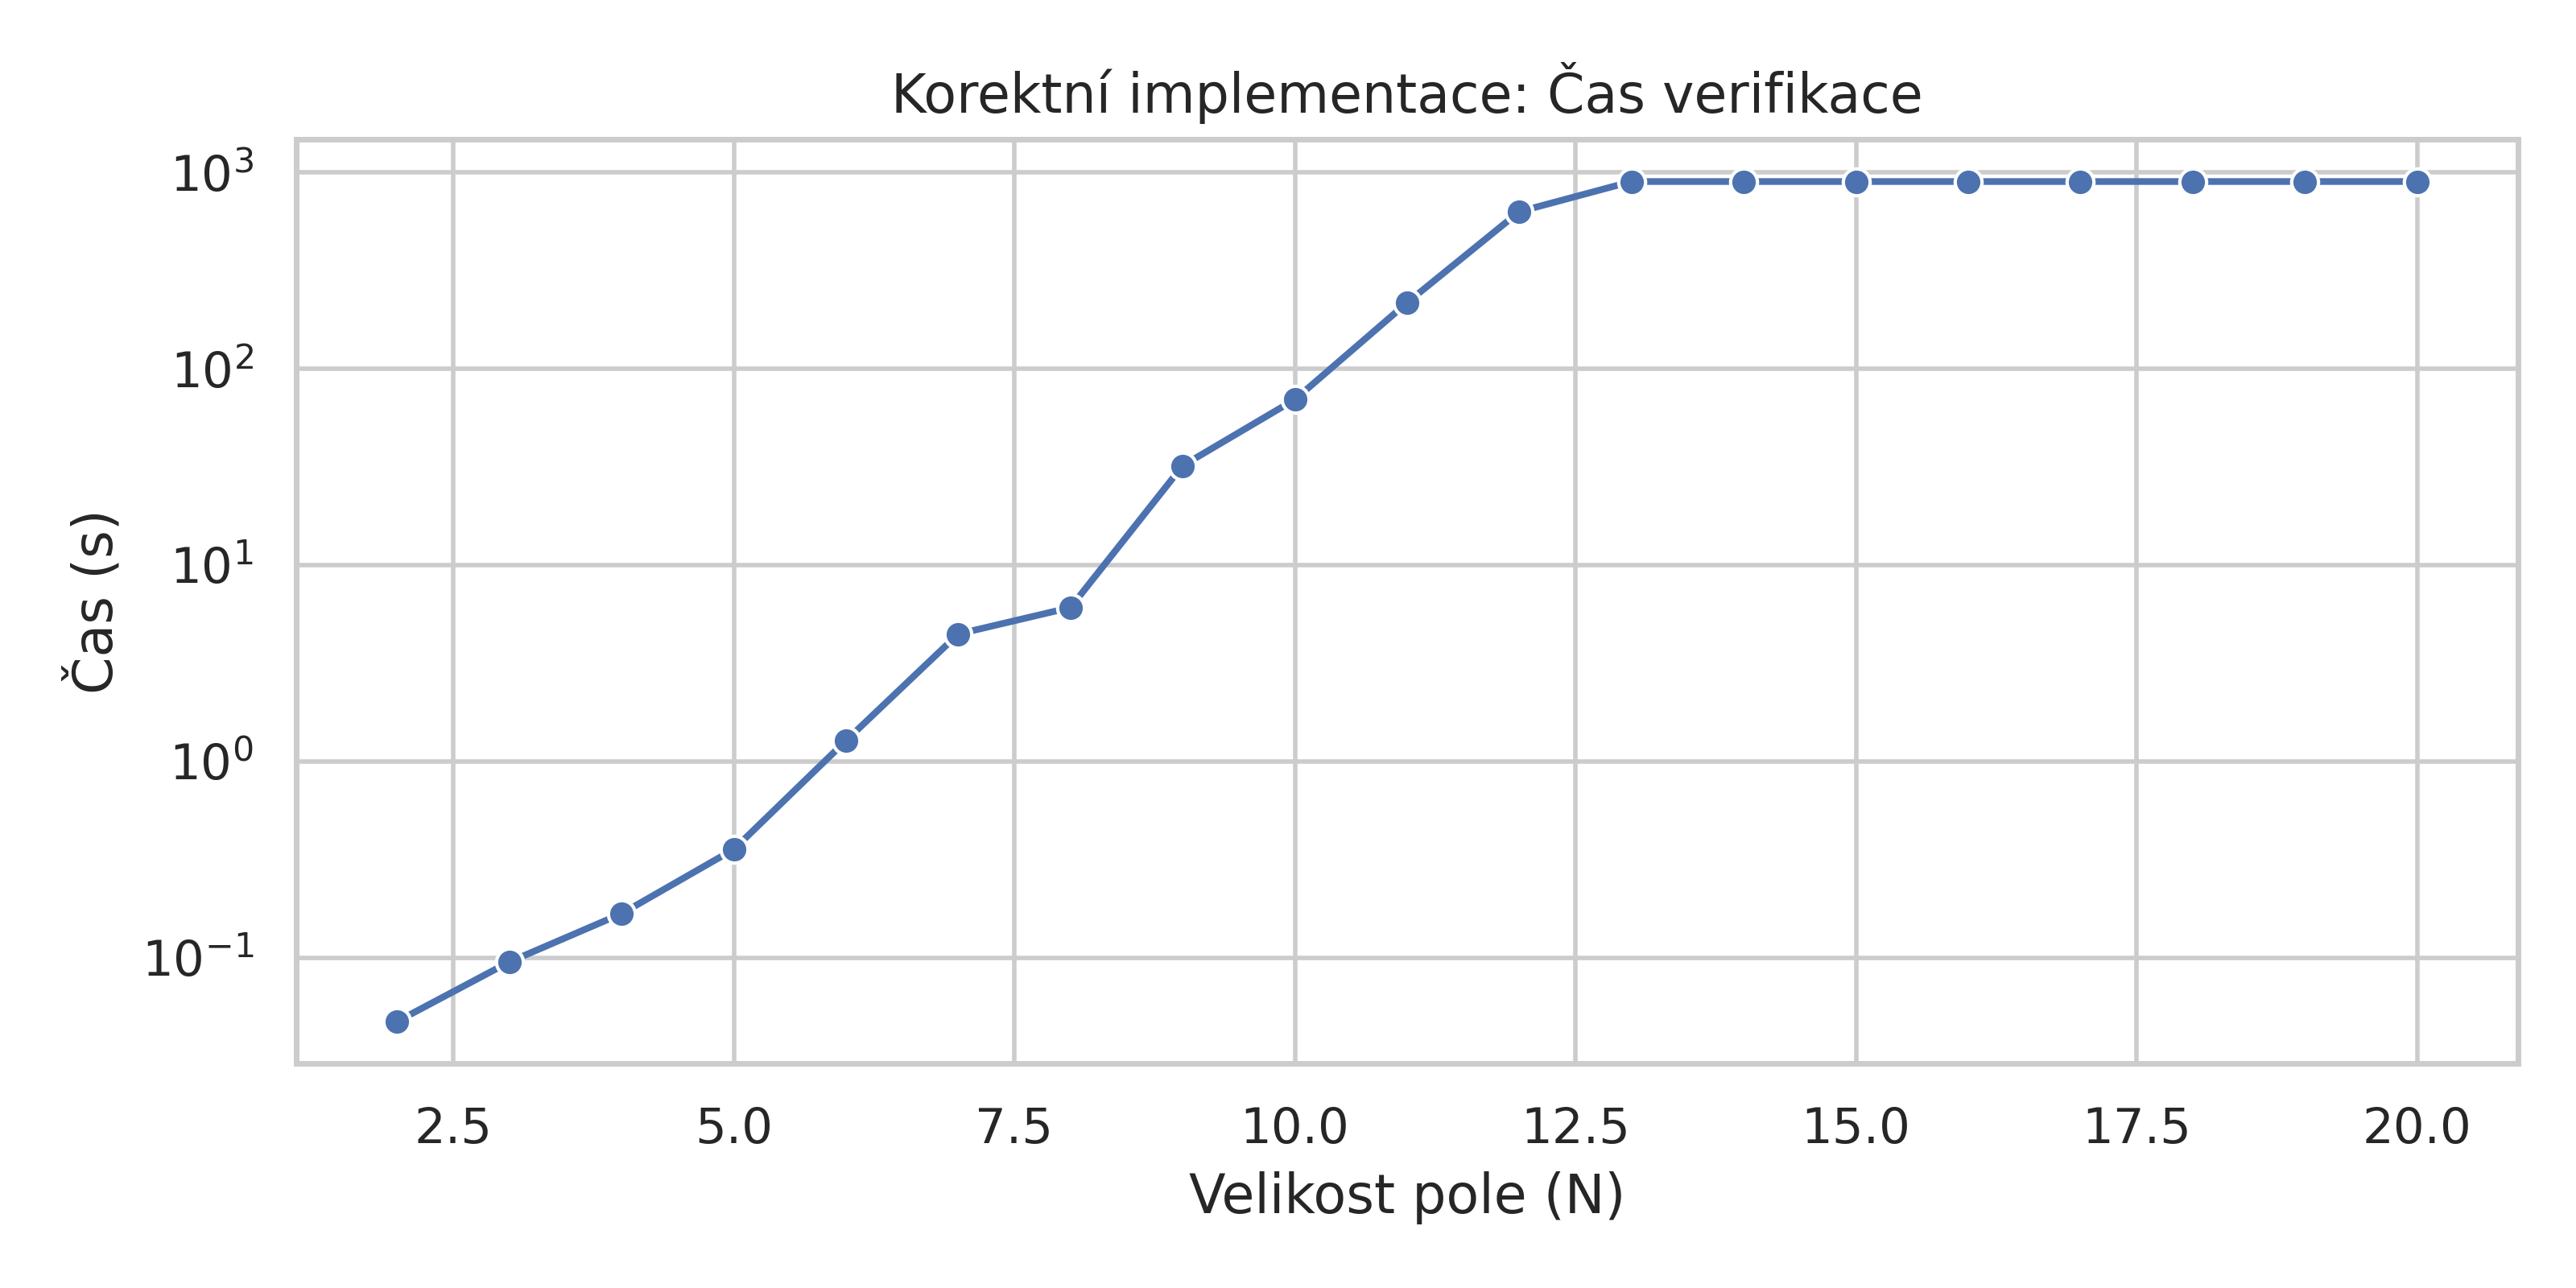
\includegraphics[width=0.8\linewidth]{img/graph_correct_total_time.png}
    \caption{Graf závislosti rychlosti verifikace na velikosti pole při verifikaci standardní implementace algoritmu Merge sort.}
    \label{fig:std_merge_sort_speed}
\end{figure}
Vertikální osa je v~logaritmickém měřítku, přičemž je patrné, že s~rostoucí velikostí pole čas verifikace velmi rychle narůstá.
Při spouštění analýzy byl nastaven timeout 15 minut; pro hodnoty $\texttt{SIZE} \geq 13$ již CBMC nebyl schopen korektnost programu v~daném časovém limitu ověřit.

Tento výsledek ilustruje praktické omezení použití bounded model checkingu pro rekurzivní algoritmy pracující s~poli (respektive pracující s~jakýmkoliv modelem, díky kterému verifikovaný model explozivně narůstá), a~to i~pro malé velikosti vstupů.

\paragraph{Velikost CNF formule.}
Na obrázku \ref{fig:std_merge_sort_formula_size} je znázorněna velikost CNF formule generované CBMC v~závislosti na velikosti vstupního pole.
\begin{figure}[h]
    \centering
    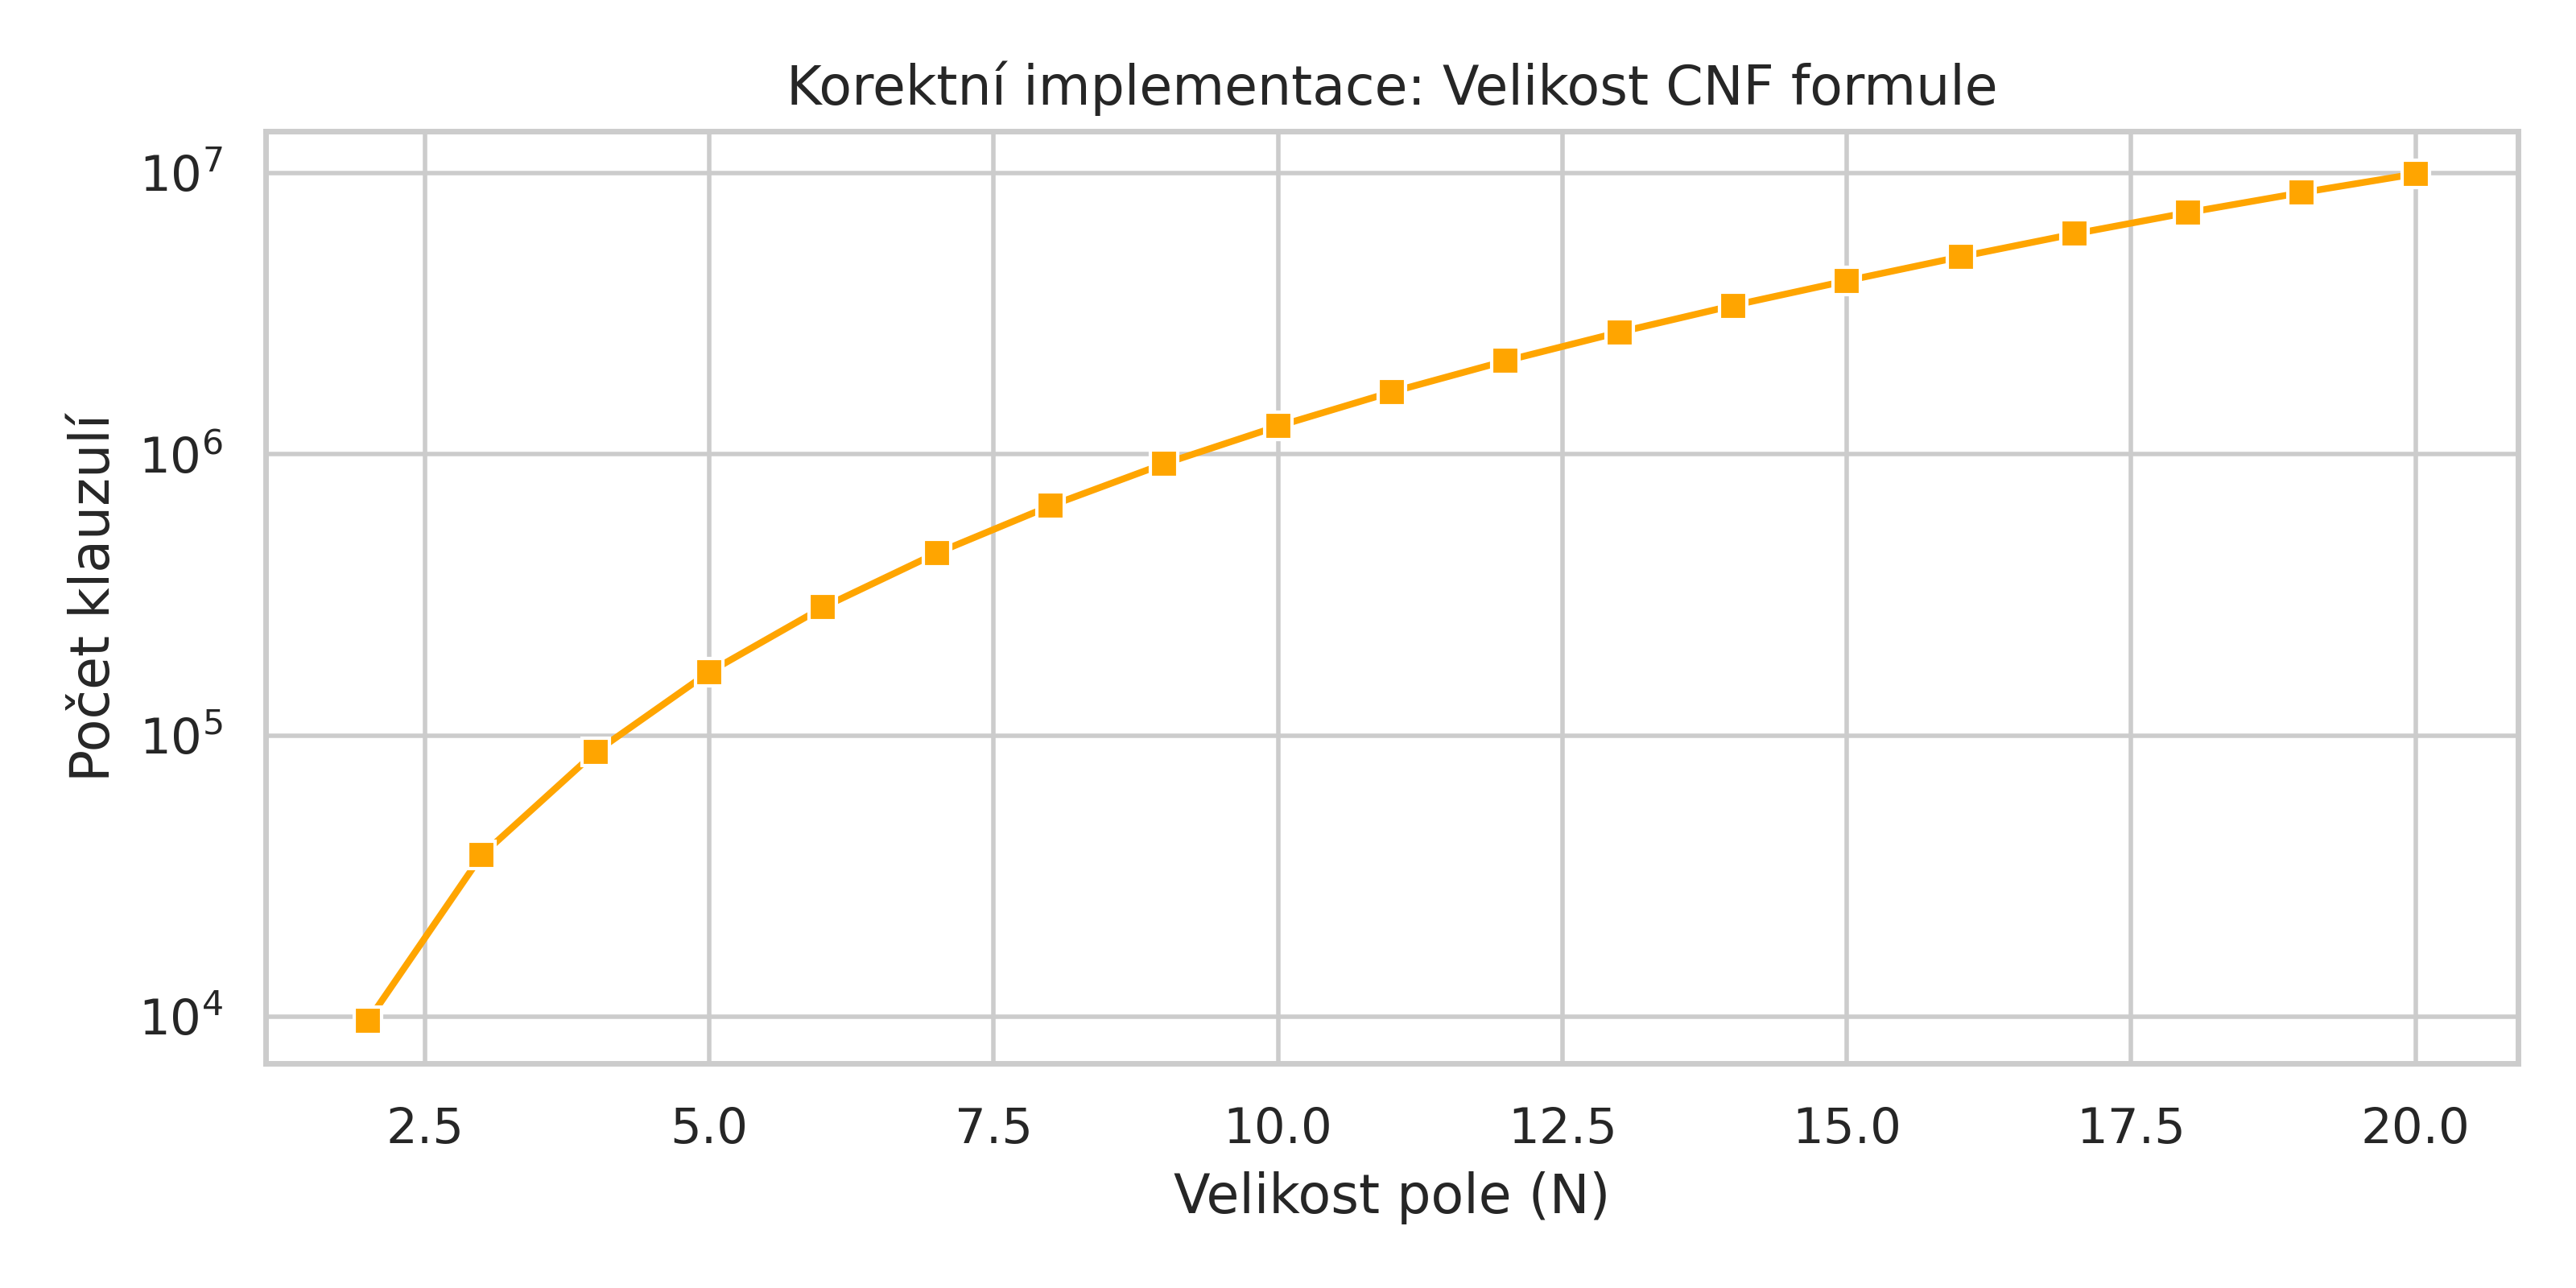
\includegraphics[width=0.8\linewidth]{img/graph_correct_clauses.png}
    \caption{Graf závislosti velikosti vygenerované CNF formule na velikosti pole při verifikaci standardní implementace algoritmu Merge sort.}
    \label{fig:std_merge_sort_formula_size}
\end{figure}
I~zde je vertikální osa v~logaritmickém měřítku.
Velikost formule roste velmi rychle a~pro $\texttt{SIZE} = 20$ se již pohybuje v~řádu milionů klauzulí.
Nárůst velikosti formule je zřetelný zejména pro menší hodnoty $\texttt{SIZE}$, kde každé zvětšení vstupu znamená výrazné rozšíření výsledné formule.

Samotná velikost formule však ještě plně nevysvětluje extrémní nárůst času verifikace, což je patrné z~následujícího rozboru jednotlivých částí verifikace.

\paragraph{Časová složitost různých fází verifikace.}
Obrázek \ref{fig:std_merge_sort_breakdown} porovnává čas strávený generováním formule pro SAT solver a~čas potřebný k~jejímu řešení.
\begin{figure}[h]
    \centering
    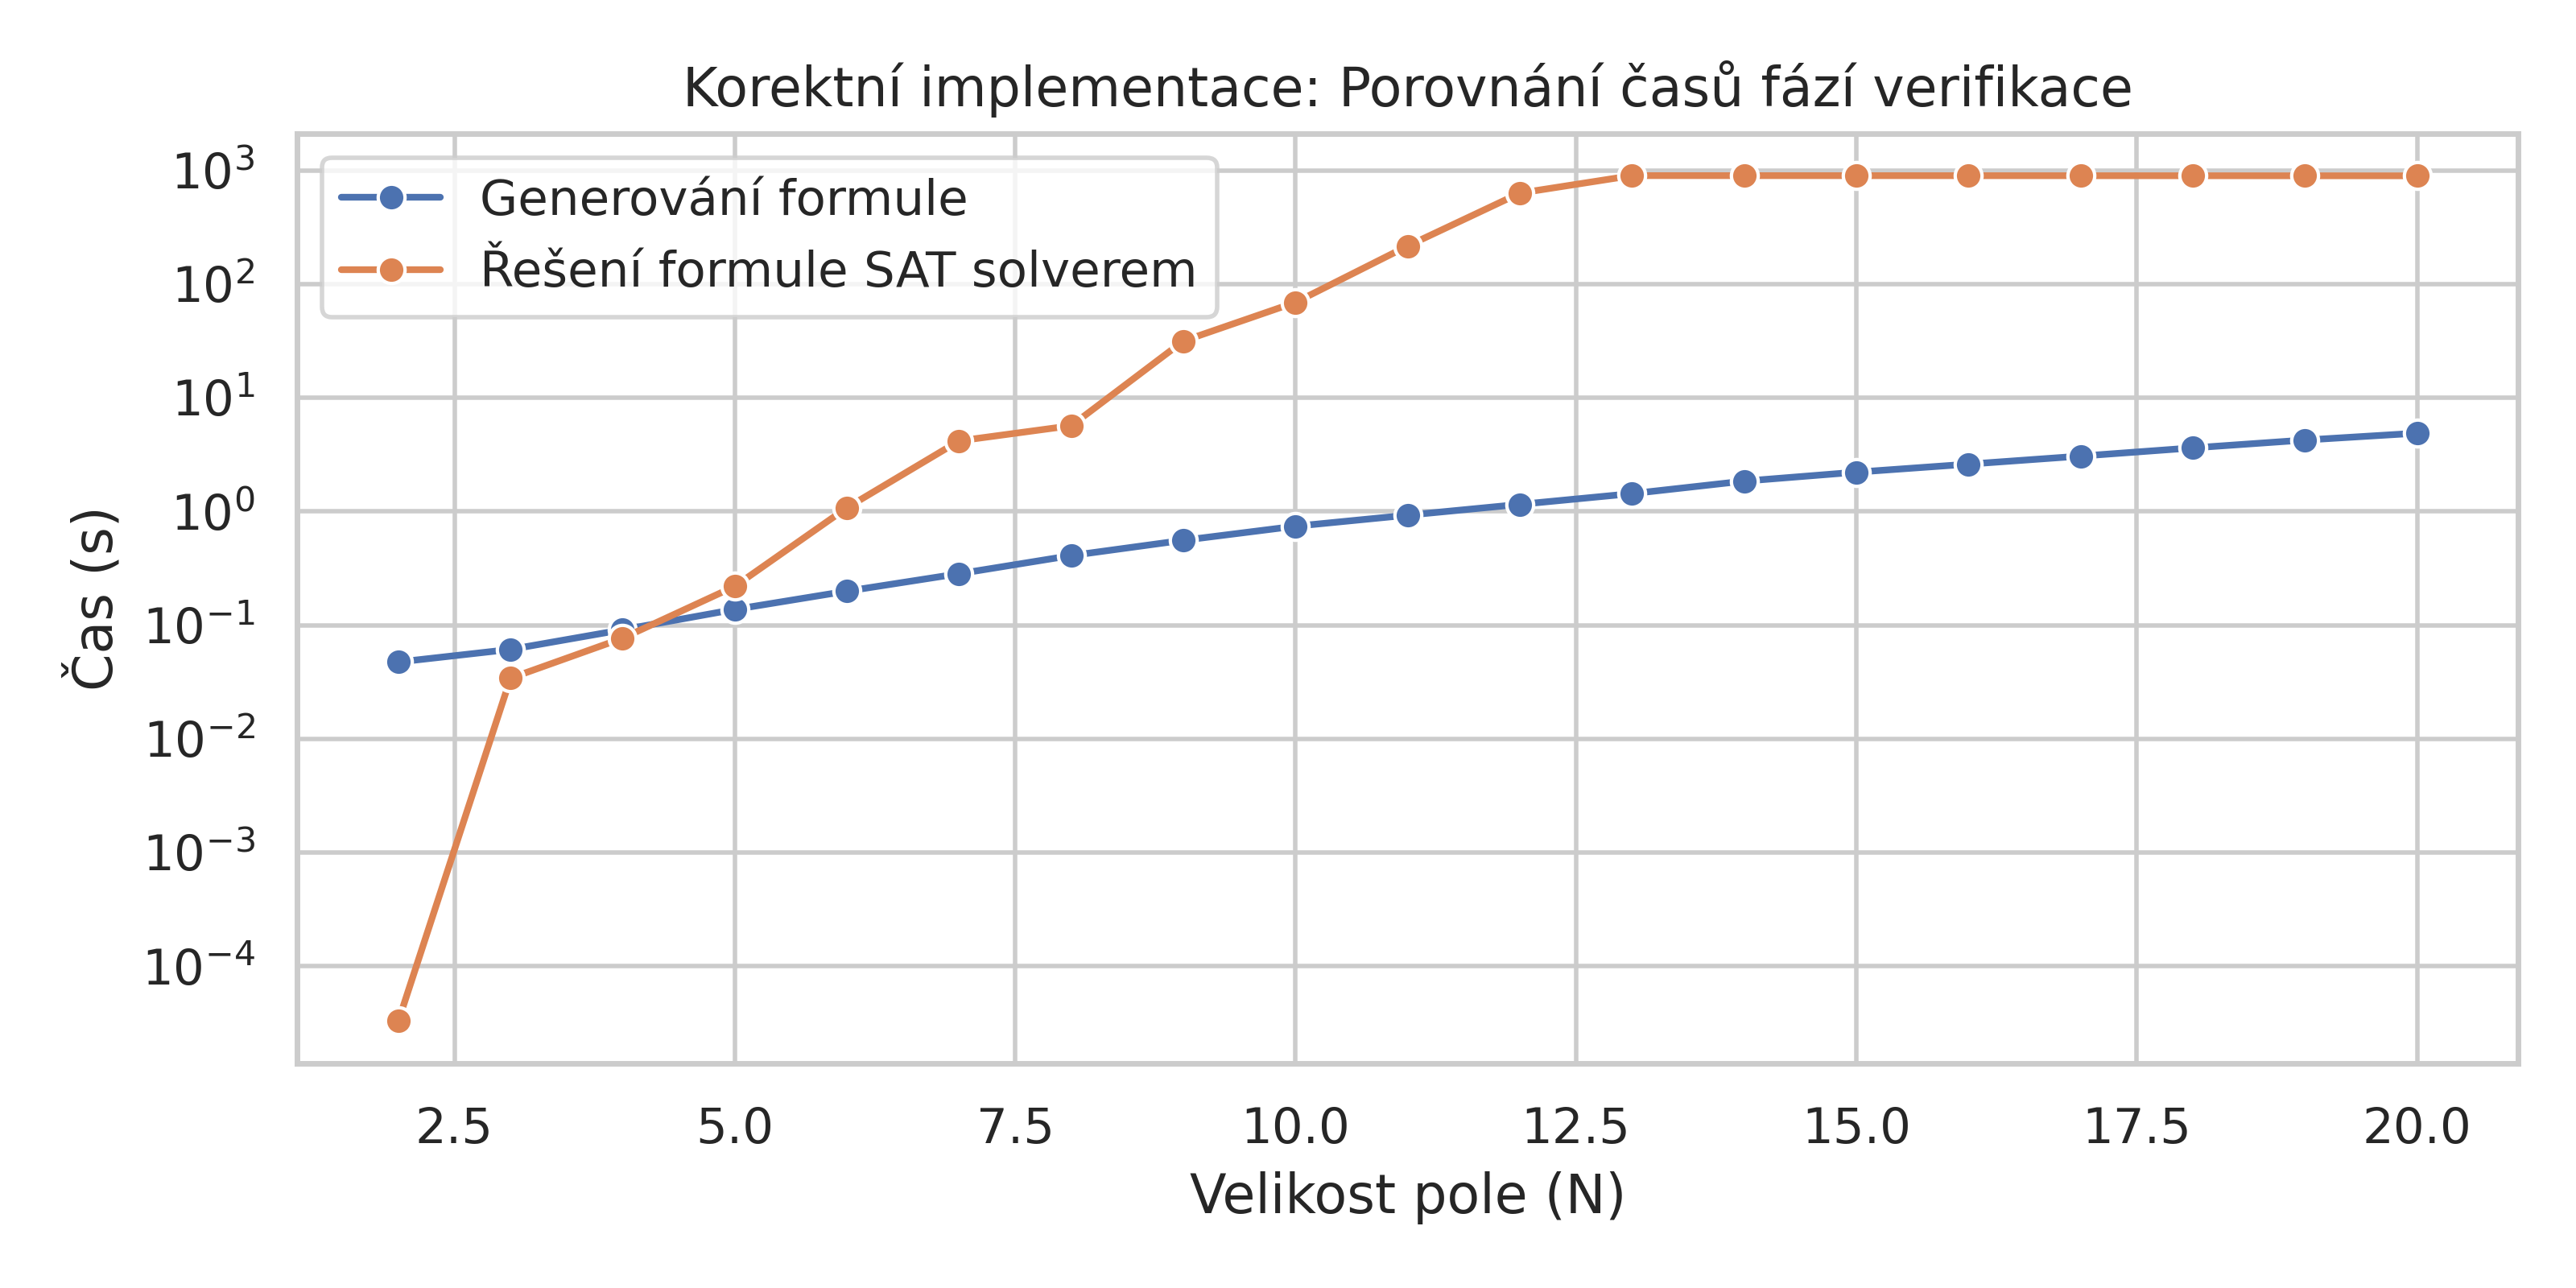
\includegraphics[width=0.8\linewidth]{img/graph_correct_breakdown.png}
    \caption{Graf srovnání časové složitosti fáze generování formule pro SAT solver a~jejím řešením při verifikaci standardní implementace algoritmu Merge sort.}
    \label{fig:std_merge_sort_breakdown}
\end{figure}
Pro malé velikosti pole ($\texttt{SIZE} \leq 4$) je dominantní fází generování formule, zatímco samotné řešení SAT problému je relativně levné.
S~rostoucí velikostí vstupu se však situace rychle obrací a~řešení formule se stává jednoznačně nejnáročnější částí verifikace.

Tento jev odpovídá očekávání: zatímco generování formule roste přibližně lineárně s~velikostí modelu, složitost řešení SAT problému je výrazně ovlivněna kombinatorickou explozí možných stavů programu.

\subsubsection{Experimenty s modifikovaným algoritmem}\label{sec:experiments_incorrect_merge_sort}

Do původního Merge sort algoritmu byly postupně vneseny dvě chyby.
První chyba spočívala v~prohození řadící podmínky na řádku \ref{code:merge_sort_bug_condition}, aby algoritmus řadil sestupně a~ne vzestupně.

Druhá modifikace simuluje implementační chybu způsobenou opomenutím závěrečné fáze algoritmu, kdy dochází ke zkopírování zbývajících prvků poté, co jedno podpole bylo plně zpracováno.
V~kódu se jedná o~řádky \ref{code:copy_remaining_start}--\ref{code:copy_remaining_end}.

\paragraph{Chyba směru řazení algoritmu.}
Pro účely prvního experimentu byla vnesena do kódu opačná podmínka pro řazení.
Jediná změna tedy proběhla na řádku \ref{code:merge_sort_bug_condition}:
\begin{center}
    \mintinline{c}{if (left_subarray[i] <= right_subarray[j])} \\*[0.5em]
    $\Downarrow$ \\*[0.5em]
    \mintinline{c}{if (left_subarray[i] > right_subarray[j])}
\end{center}
Z~hlediska výpočetní náročnosti by se tento experiment neměl lišit od verifikace korektní implementace.
Předpokládáme, že SAT formule bude přibližně stejně velká, protože během zpracování kódu se vygenerují přibližně stejné klauzule, jen podmínky v~guardech budou opačné pro ekvivalentní \texttt{if} příkazy.
Může ale nastat situace, kdy SAT solver najde ohodnocení proměnných vedoucí ke splnitelnosti rychleji než důkaz, že žádná kombinace vstupních proměnných ke splnitelnosti nevede.
To ale závisí na vnitřním algoritmu SAT solveru, protože existují různé heuristiky, které tyto nástroje implementují.

Nejdříve ověříme velikost SAT formule vzhledem k~velikosti pole, pro které se kód ověřuje.
To je ukázáno na obrázku~\ref{fig:MergeSort_CondBug_FormulaSize}.
\begin{figure}[h]
    \centering
    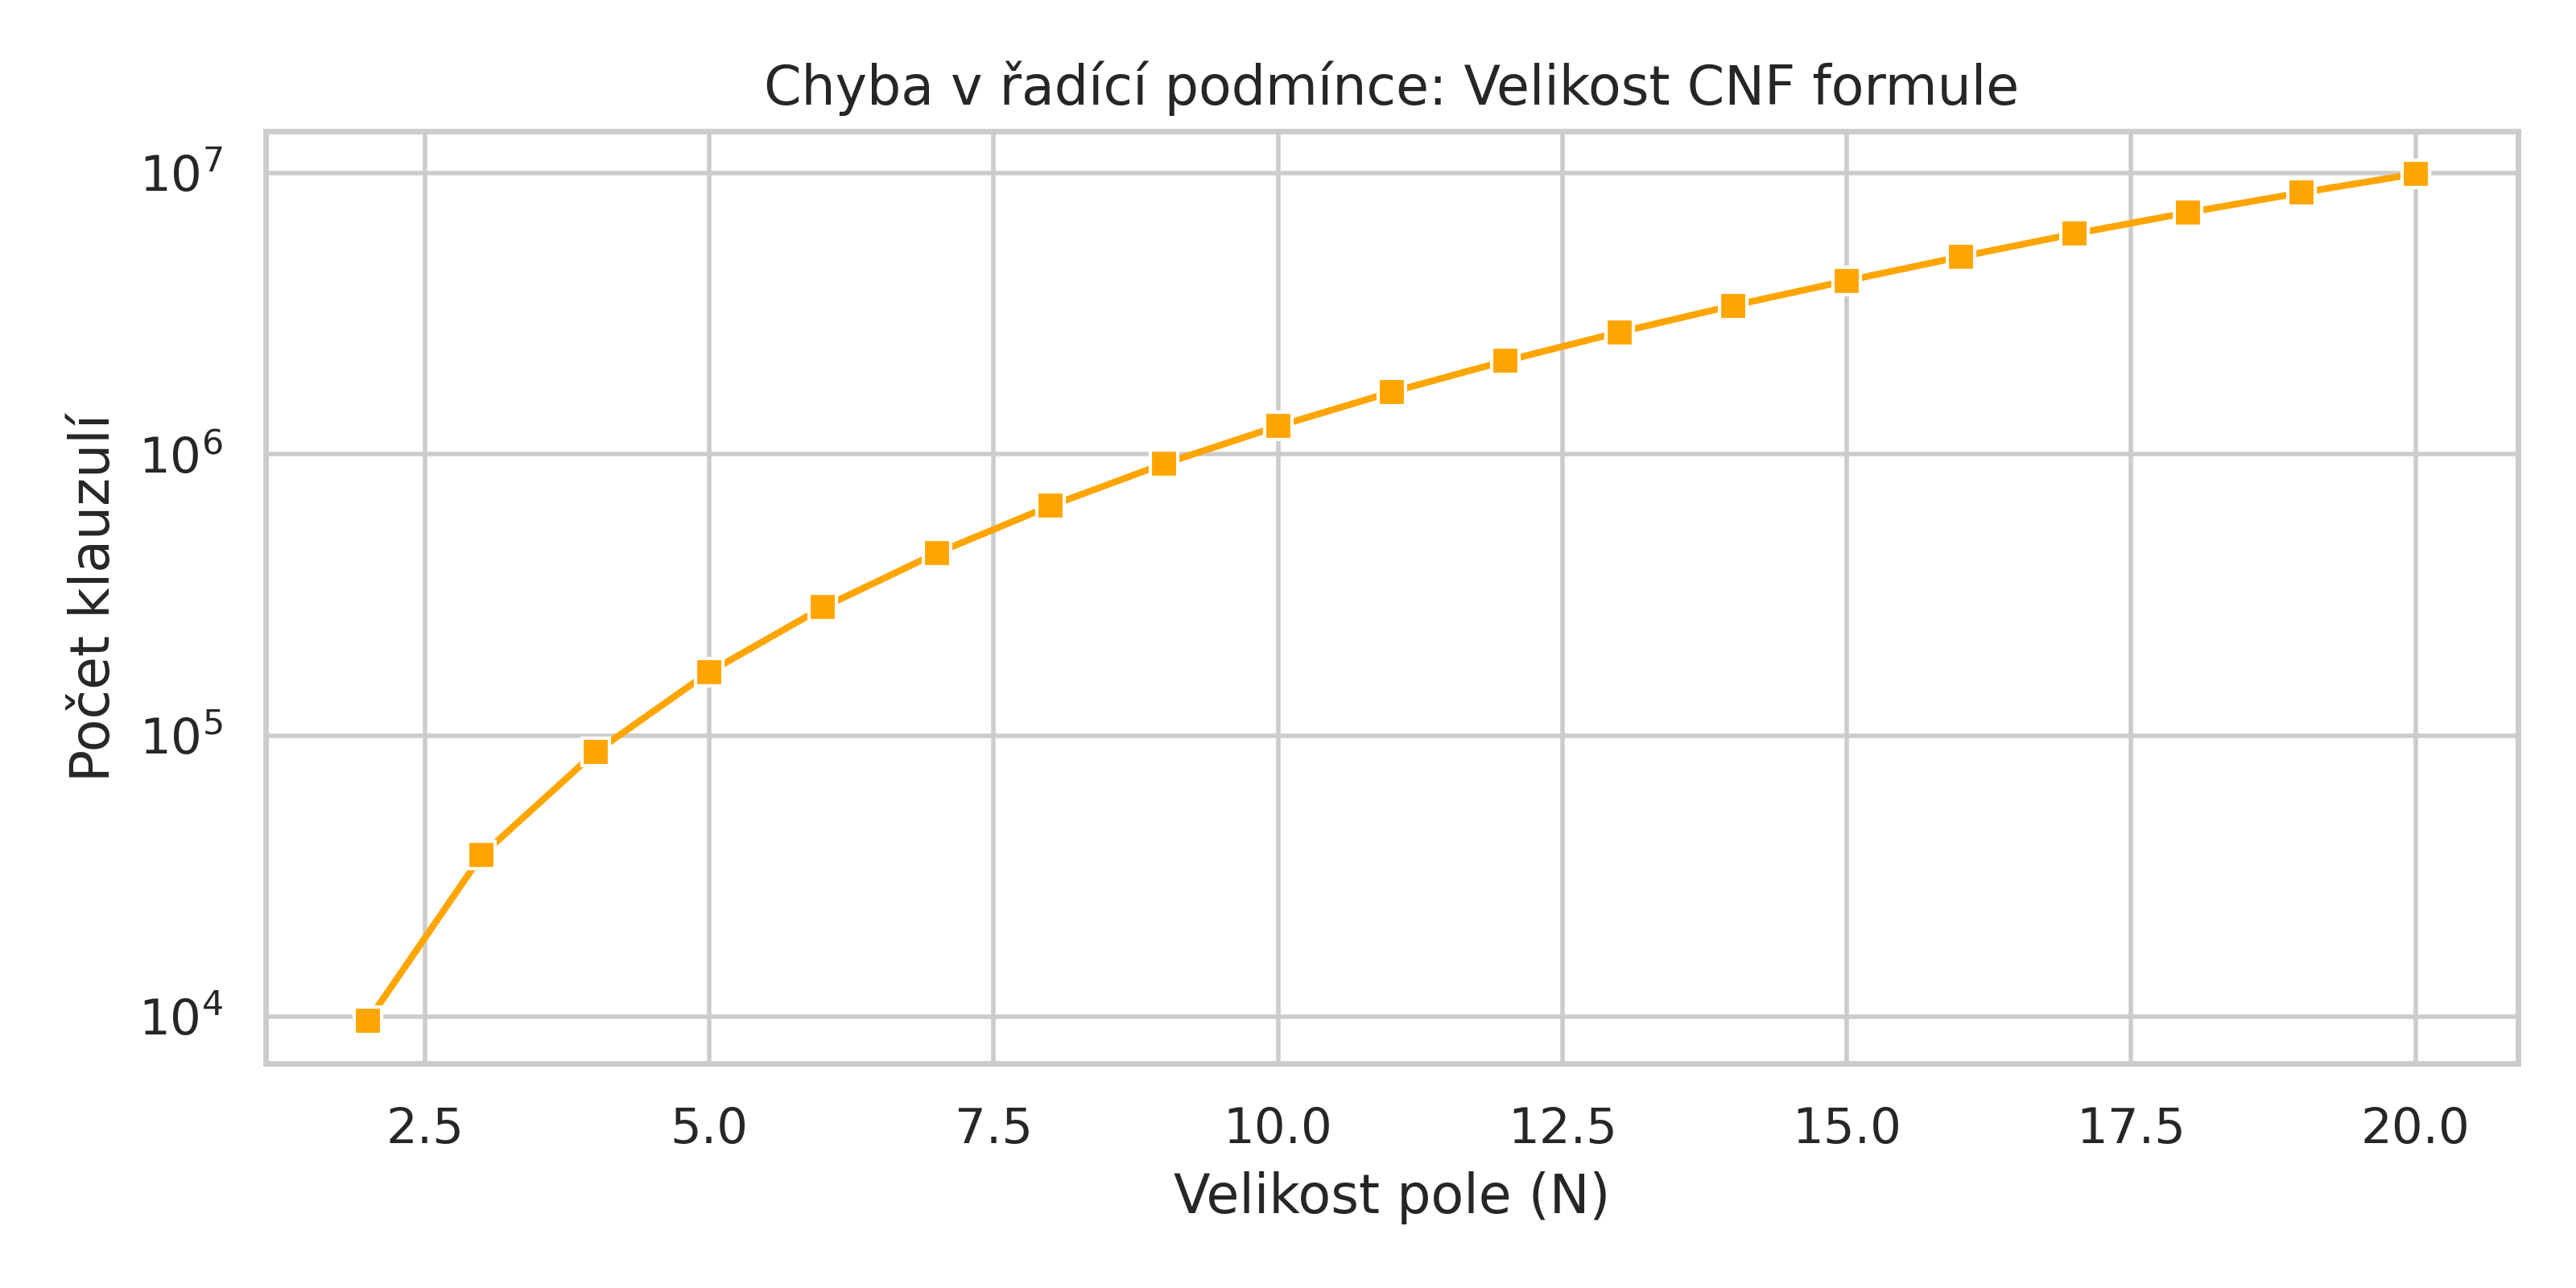
\includegraphics[width=0.8\linewidth]{img/graph_cond_clauses.png}
    \caption{Graf závislosti velikosti formule na velikosti pole při obrácení řadící podmínky.}
    \label{fig:MergeSort_CondBug_FormulaSize}
\end{figure}
Vidíme, že velikost generovaných formulí se prakticky nezměnila, což potvrzuje naši hypotézu.
Druhé případné zrychlení by mohlo nastat v~situaci, kdy formule má příznivou strukturu pro SAT solver.
Časové výsledky verifikace jsou na obrázku~\ref{fig:MergeSort_CondBug_Speed}.
\begin{figure}[ht]
    \centering
    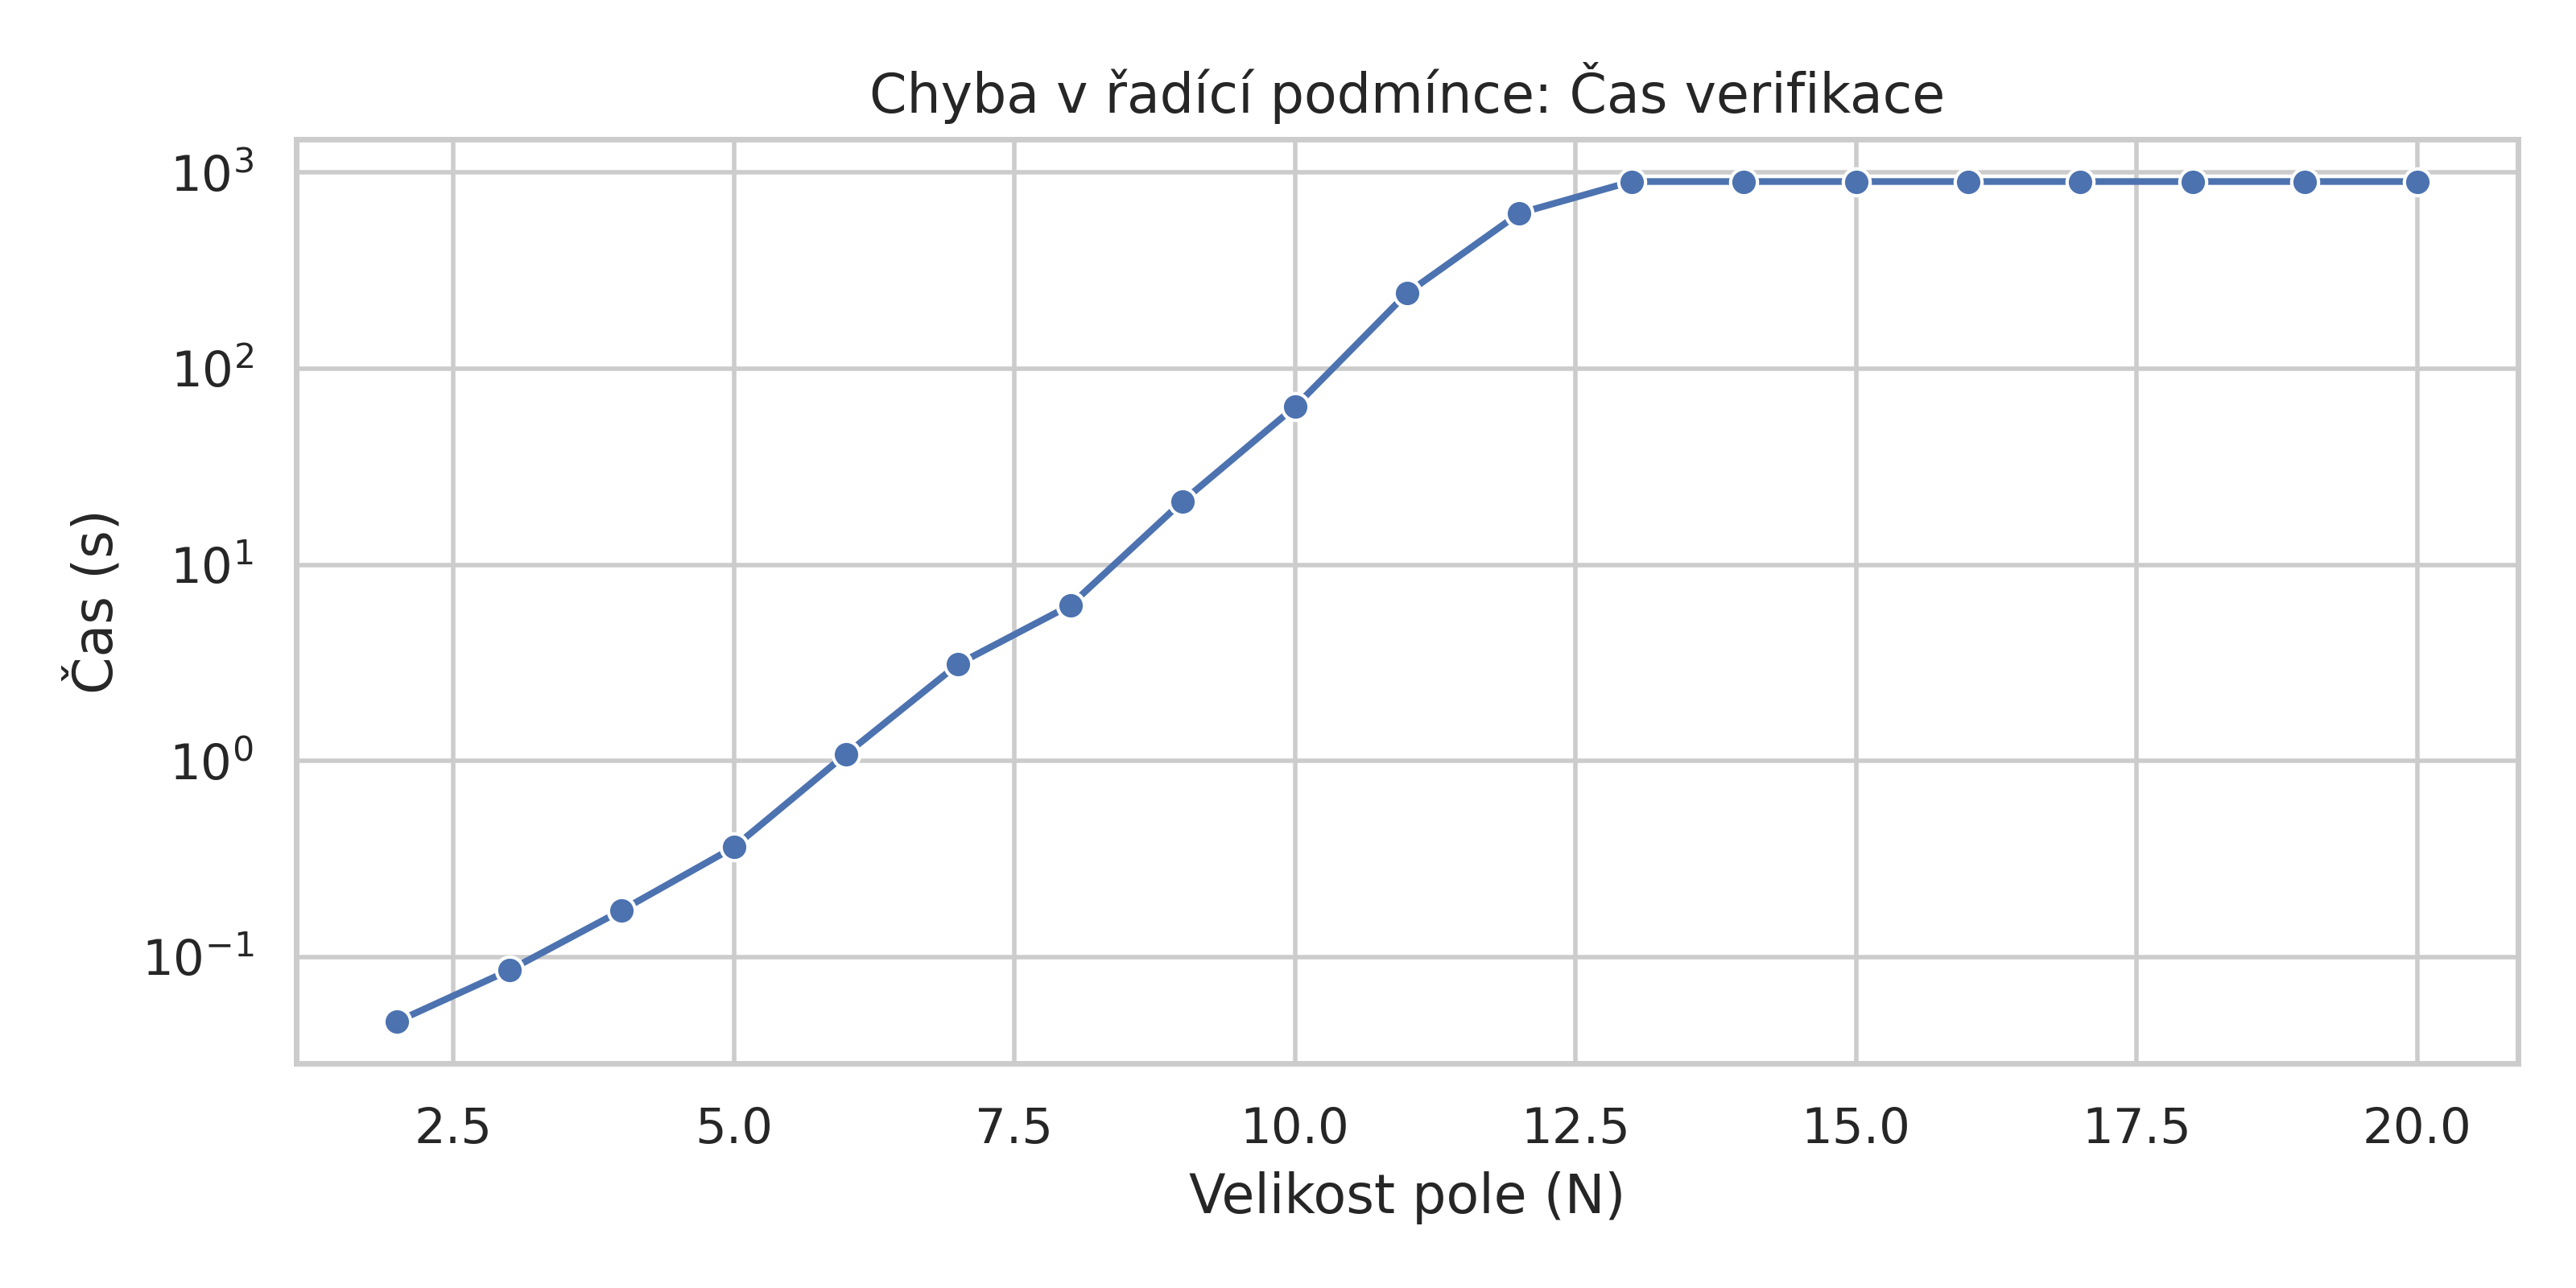
\includegraphics[width=0.8\linewidth]{img/graph_cond_total_time.png}
    \caption{Graf závislosti rychlosti verifikace na velikosti pole při obrácení řadící podmínky.}
    \label{fig:MergeSort_CondBug_Speed}
\end{figure}

Ani rychlost verifikace se nezměnila, což značí velmi podobnou strukturu formule.
Tato chyba tedy verifikaci prakticky nijak neovlivnila.
Stále trvá velmi dlouho, pro větší pole se tento problém stává prakticky neřešitelným v~rozumném čase.
Dá se tedy předpokládat, že budou i~podobné časové poměry mezi generováním formule a~jejím řešením; tato hypotéza je potvrzena na obrázku~\ref{fig:MergeSort_CondBug_Breakdown}.
\begin{figure}[h]
    \centering
    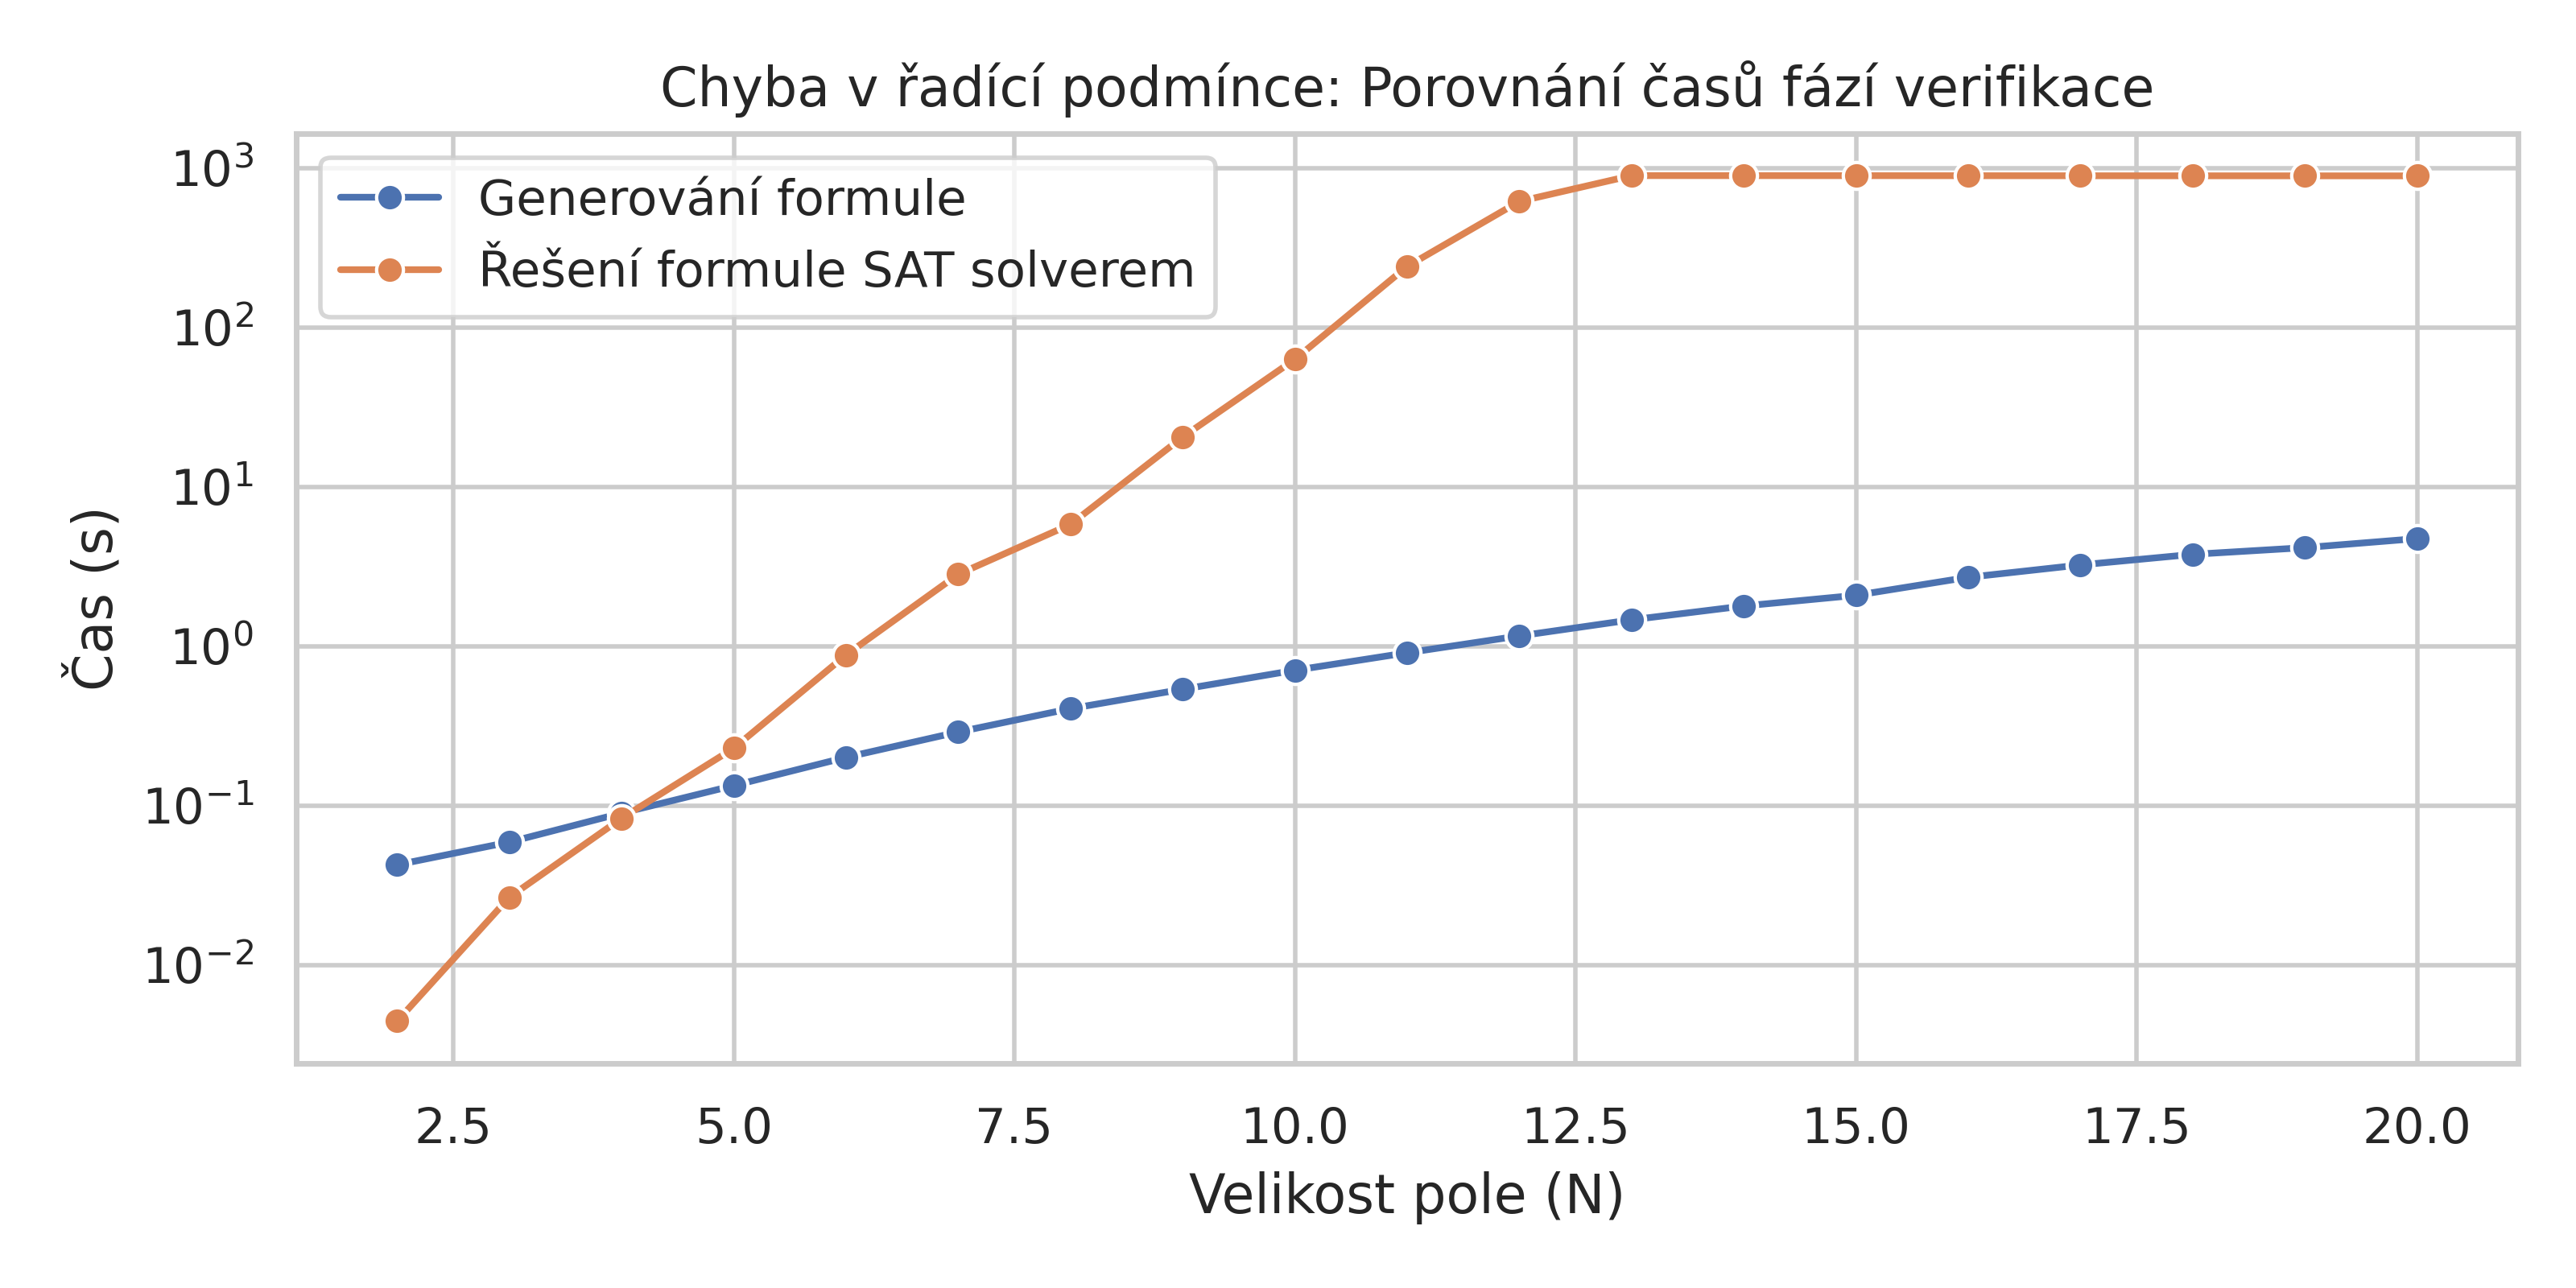
\includegraphics[width=0.8\linewidth]{img/graph_cond_breakdown.png}
    \caption{Graf srovnání rychlosti fáze generování formule pro SAT solver a jejího řešení při verifikaci Merge sortu s~obrácenou řadící podmínkou.}
    \label{fig:MergeSort_CondBug_Breakdown}
\end{figure}

\paragraph{Chyba opomenutí závěrečné fáze algoritmu.}
Druhou uměle vnesenou chybou je smazání cyklů na řádcích \ref{code:copy_remaining_start}--\ref{code:copy_remaining_end}.
Budeme se především zabývat otázkou, jak se tato změna projeví na době analýzy algoritmu.
V~případě korektní implementace nebo prohození směru řazení analýza trvala přibližně stejnou dobu, a~to neúnosně dlouhou.
Druhá modifikace je větší zásah do struktury algoritmu.
Odstranění závěrečných slučovacích smyček vede k~tomu, že podpole vzniklá slučováním jsou zjevně nekorektní, což by se mohlo projevit i~na průběhu verifikace.
CBMC neposuzuje sémantickou zjevnost chyby, ale generuje SAT formuli, která program reprezentuje.
Ta bude menší, protože jsou odstraněny dva cykly, které by se jinak rozbalovaly při každém rekurzivním volání funkce \texttt{Merge()}.
Výsledná SAT formule tím pádem obsahuje méně proměnných i~klauzulí a~její řešení může být pro SAT solver snazší.
Nicméně doba analýzy stále záleží na řešitelnosti dané formule.

Pro druhou modifikaci algoritmu proto očekáváme zrychlení verifikace.
Nejprve si ověříme, že generovaná formule je opravdu menší.
Velikosti formulí vůči velikostem ověřovaných polí jsou na obrázku~\ref{fig:MergeSort_MergeBug_FormulaSize}.
\begin{figure}[h]
    \centering
    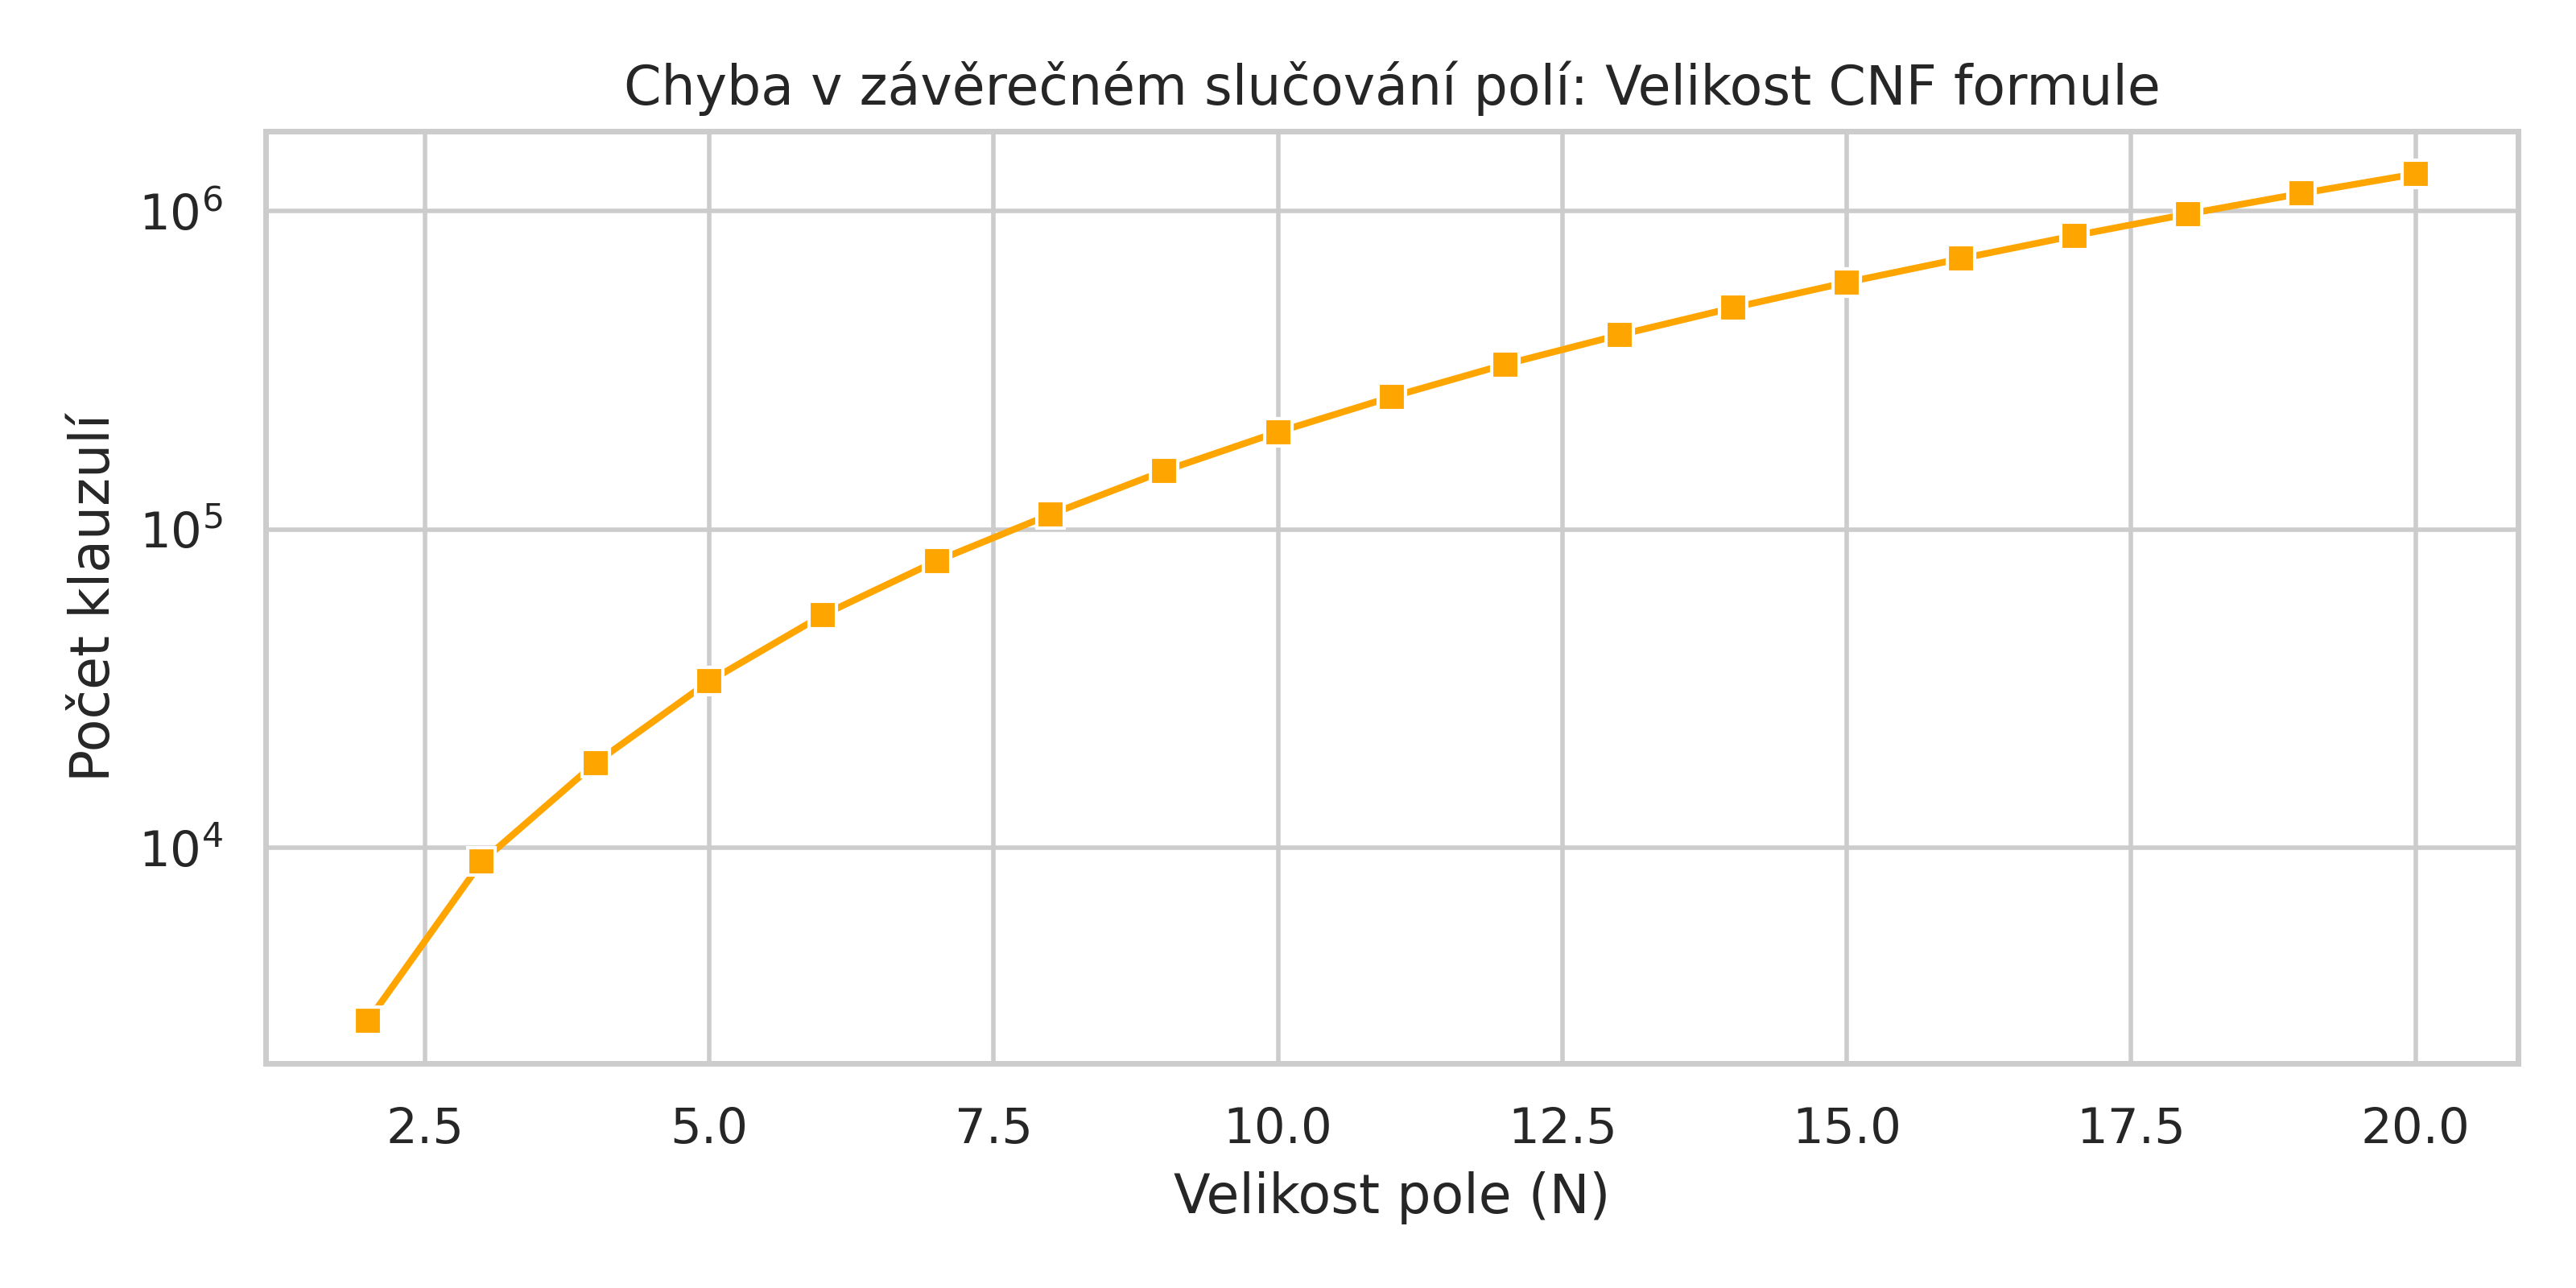
\includegraphics[width=0.8\linewidth]{img/graph_array_clauses.png}
    \caption{Graf závislosti velikosti formule na velikosti pole při odstranění závěrečných slučovacích smyček ve funkci \texttt{Merge()}.}
    \label{fig:MergeSort_MergeBug_FormulaSize}
\end{figure}

Generované formule jsou opravdu řádově menší.
Vzhledem k~exponenciálnímu nárůstu výpočetní složitosti řešení SAT formule v~závislosti na její velikosti můžeme předpokládat, že doba verifikace se také řádově sníží.
Výsledek je na obrázku~\ref{fig:MergeSort_MergeBug_Speed}.
\begin{figure}[h]
    \centering
    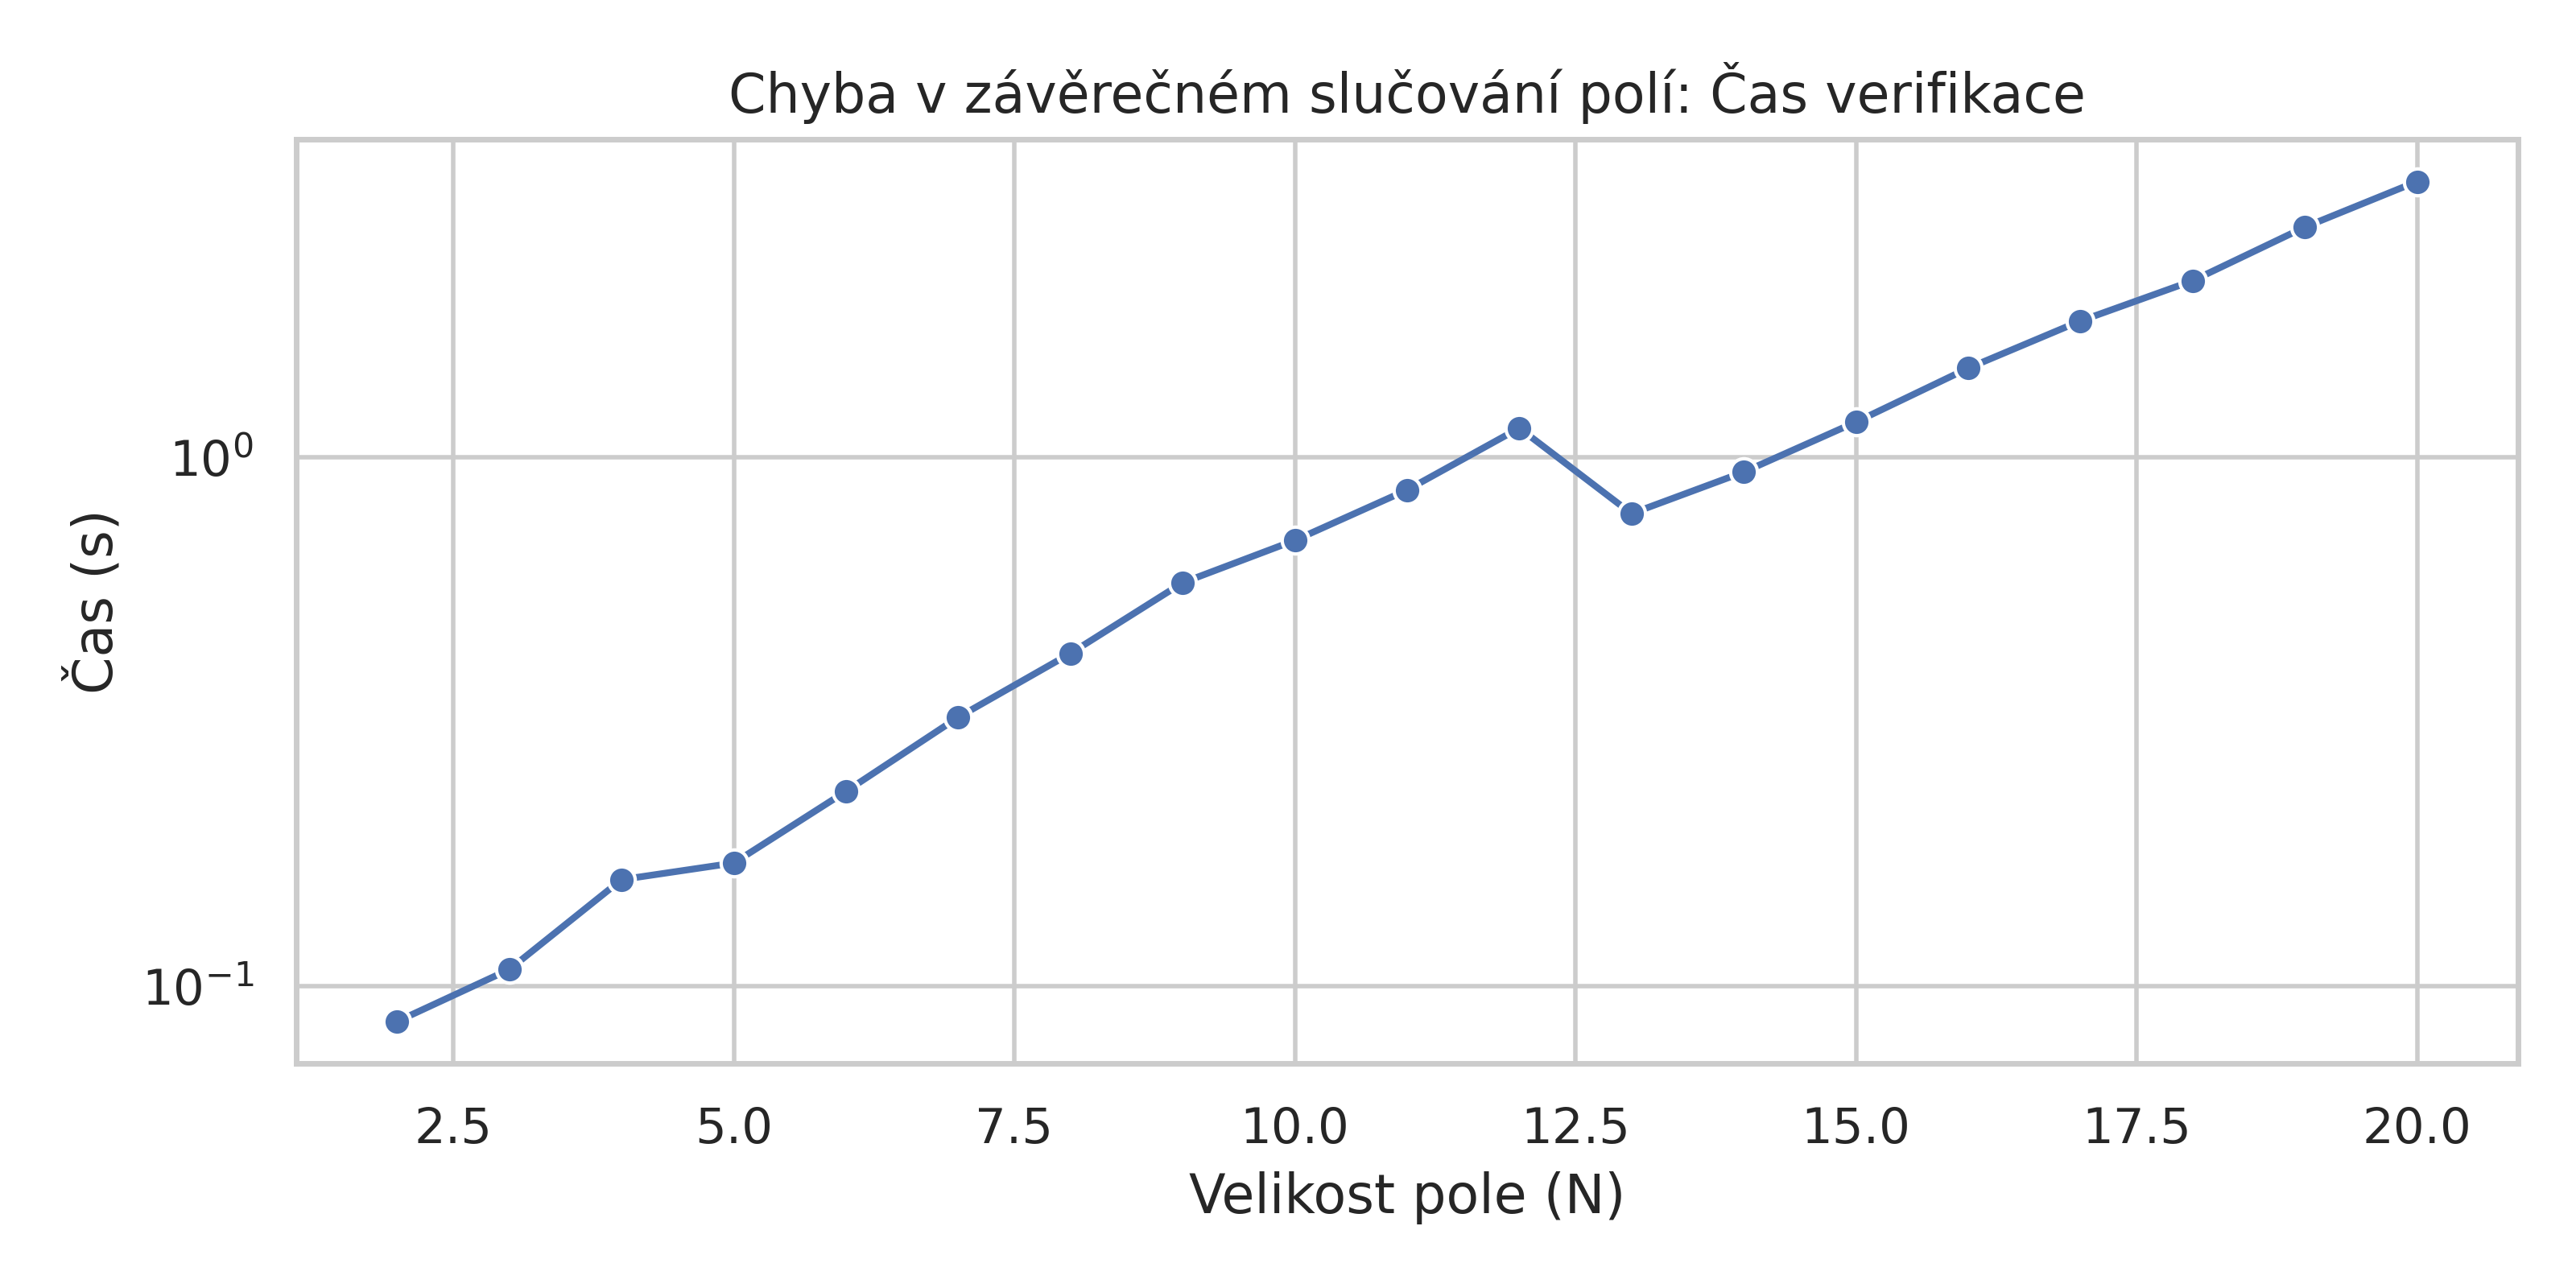
\includegraphics[width=0.8\linewidth]{img/graph_array_total_time.png}
    \caption{Graf závislosti rychlosti verifikace na velikosti pole při odstranění závěrečných slučovacích smyček ve funkci \texttt{Merge()}.}
    \label{fig:MergeSort_MergeBug_Speed}
\end{figure}

Vidíme, že rychlost verifikace se zvýšila dokonce o~několik řádů a~všechny verifikované instance byly vyřešeny relativně rychle.
Dokonce si můžeme povšimnout, že pole o~velikosti 13 bylo vyřešeno rychleji než pole o~velikosti 12, což značí, že struktura formule byla pro SAT solver příznivější a~byl schopen ji rychleji vyřešit.

Tento experiment má zajímavé výsledky i~v~rámci porovnání rychlosti generování formule a~jejím řešením, protože jednotlivé instance formulí jsou SAT solverem vyřešeny poměrně rychle.
Graficky jsou časy znázorněny na obrázku~\ref{fig:MergeSort_MergeBug_Breakdown}.
\begin{figure}[h]
    \centering
    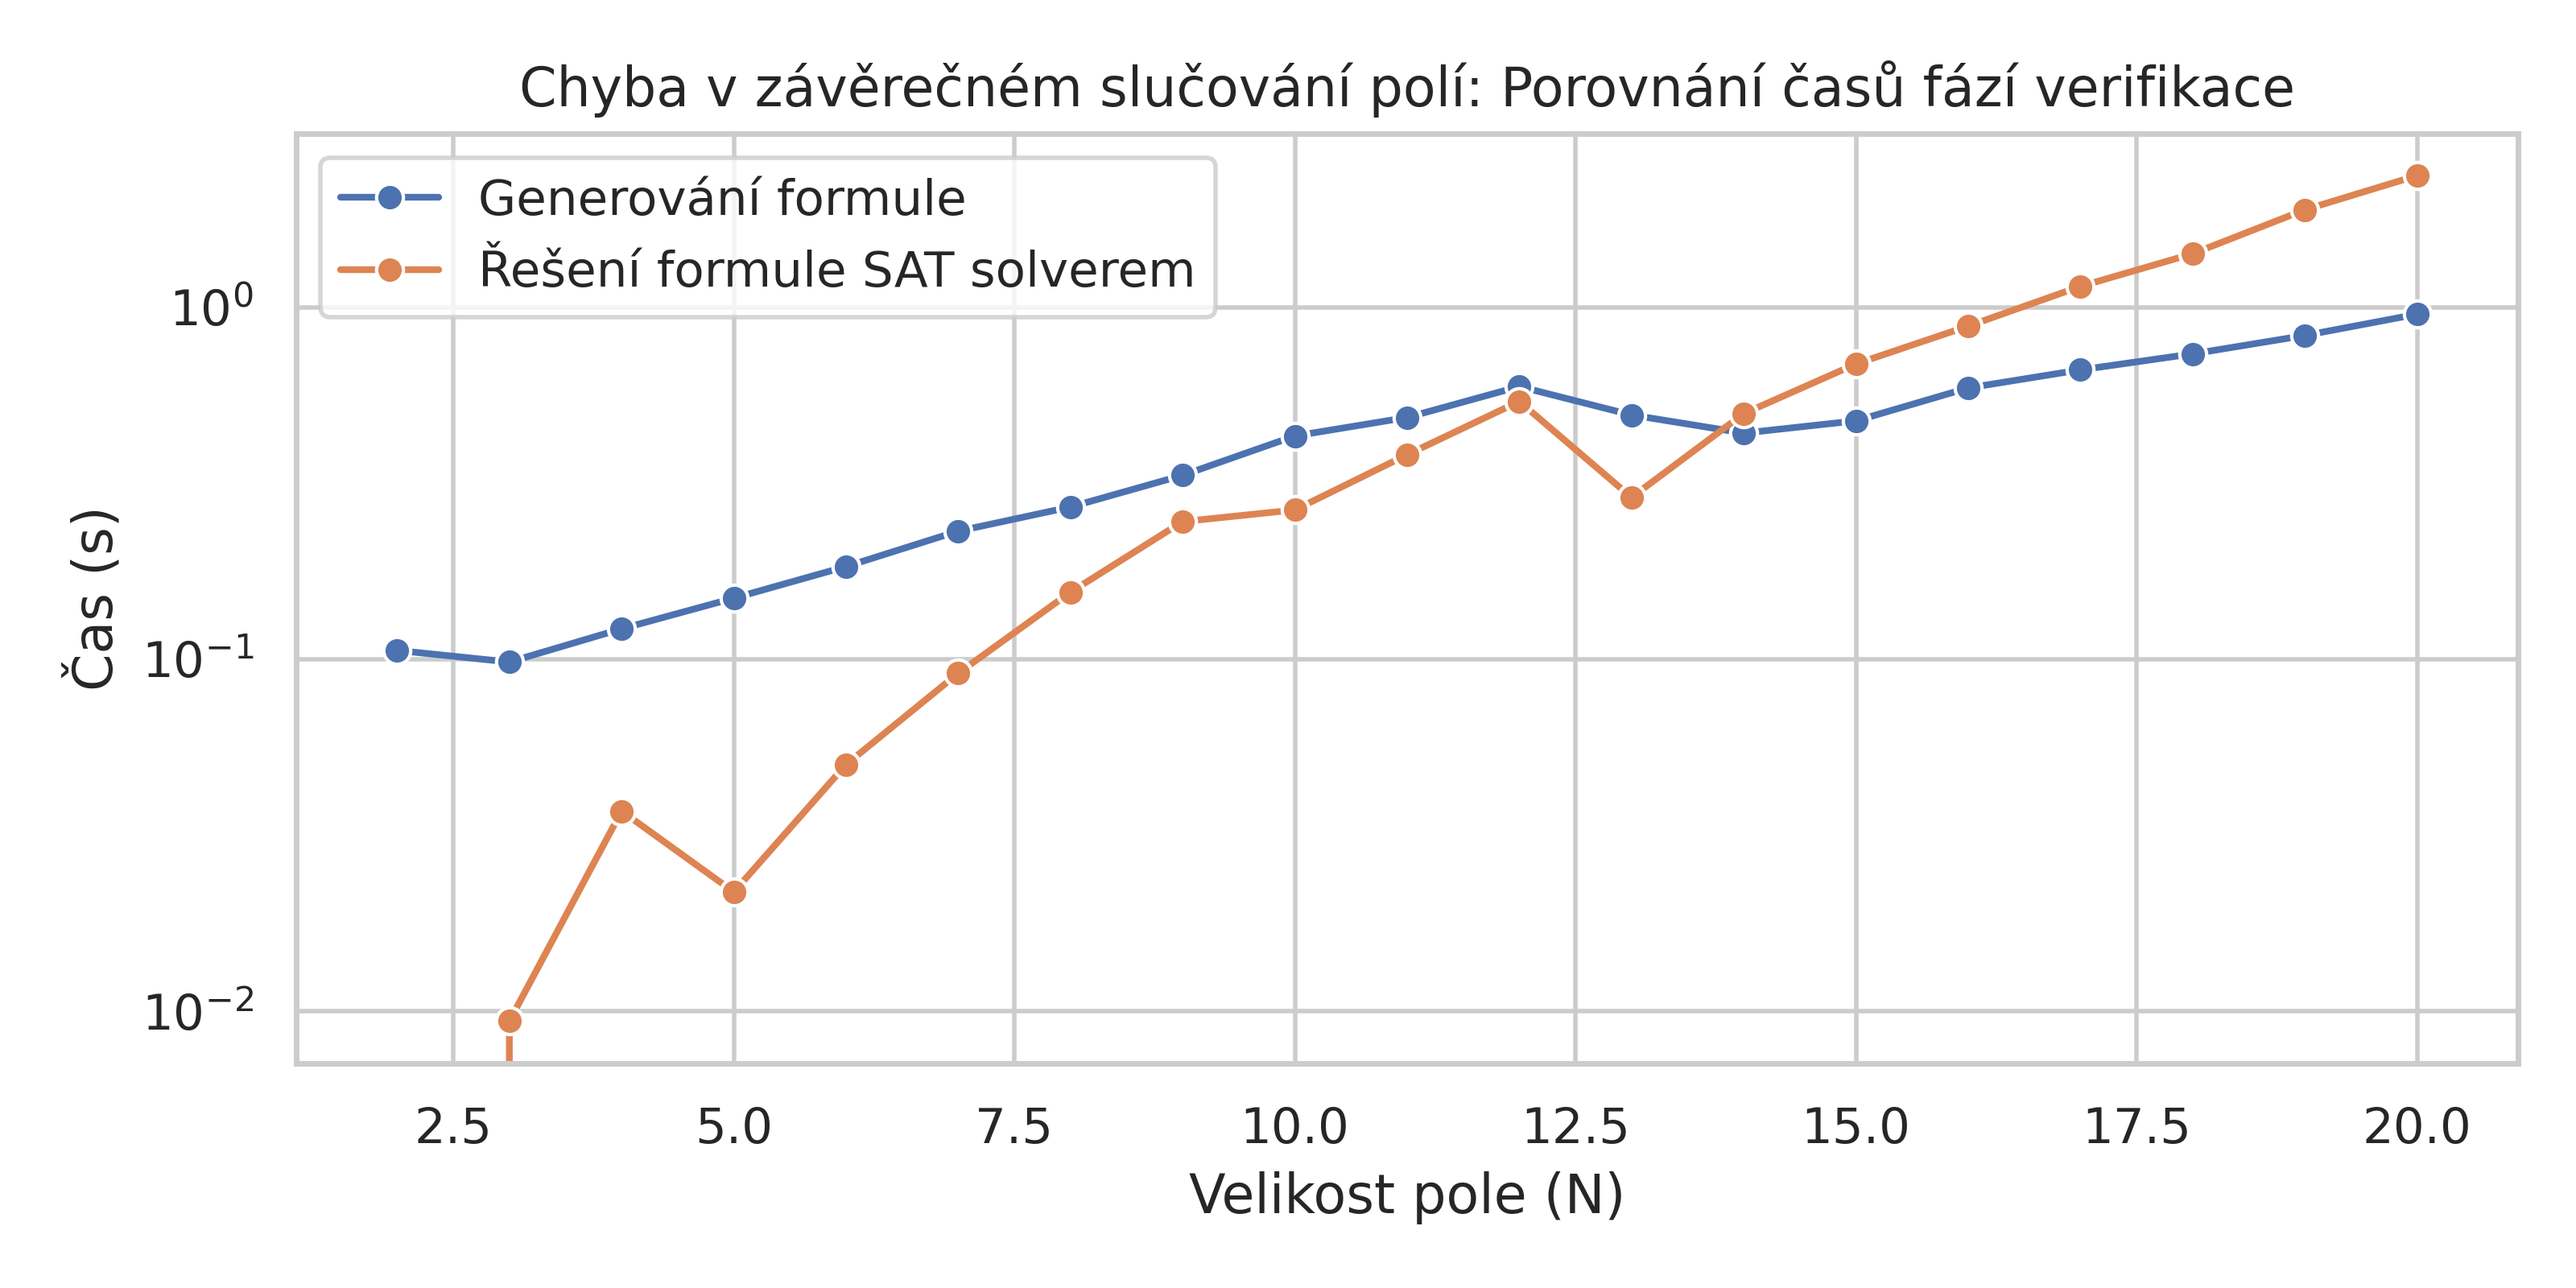
\includegraphics[width=0.8\linewidth]{img/graph_array_breakdown.png}
    \caption{Graf srovnání rychlosti fáze generování formule a jejího řešení při verifikaci algoritmu Merge sort s~opomenutým slučováním zbytků polí.}
    \label{fig:MergeSort_MergeBug_Breakdown}
\end{figure}

\subsubsection{Diskuze omezení a škálovatelnosti}\label{sec:discussion_limitations}
V~sekci \ref{sec:CBMC_Demo_MergeSort} jsme ověřovali, jak funguje technika bounded model checkingu pro algoritmus reálného charakteru.
Pro experimenty byl záměrně zvolen algoritmus Merge sort, protože je rekurzivní a~pracuje s~pomocnými poli, přičemž obě tyto programovací techniky jsou pro bounded model checking velmi komplikované na ověřování vlivem exploze stavového prostoru.
Verifikovali jsme algoritmus v~korektní implementaci a~také algoritmy modifikované s~vnesenými dvěma chybami.
Výsledky verifikací byly očekávané, tedy pro korektní algoritmus verifikace hlásila úspěch, pro nekorektní algoritmy hlásila neúspěch.

Verifikace tohoto algoritmu trvala velmi dlouhou dobu, jak jsme si ukázali v~grafech.
Kvůli explozi stavového prostoru se velikost generovaných formulí exponenciálně zvyšovala a~pro relativně malá pole formule obsahovaly i~několik milionů klauzulí.

Z~toho plyne, že tato technika je obtížně aplikovatelná pro rozsáhlé softwarové systémy, které mohou mít miliony řádků kódu.
Tento nástroj byl ale vyvinut pro verifikaci vestavěných systémů a~kritických komponent, kde je kladen extrémní důraz na korektnost implementace.
Bounded model checking s~jistotou ověří, že daný program neobsahuje chyby v~rámci uvažovaného stavového prostoru (hloubka rozbalení $k$).
Proto je používán pro verifikaci stěžejních modulů a~segmentů kódu, jejichž spolehlivost je klíčová.
Tohoto paradigmatu se budeme držet i~v~následující kapitole.

\section{Experimenty s CBMC na komplexnějších programech}\label{sec:CBMC_Experiments}
Tato kapitola bude zaměřena na verifikaci vybraných školních projektů.
Jak bylo zmíněno v~předešlé kapitole, aplikace CBMC na rozsáhlejší softwarová díla vyžaduje pečlivý výběr verifikovaných komponent kvůli výpočetní náročnosti.
Navíc nástroj nativně nepodporuje systémová volání jako jsou například funkce \texttt{scanf()}, jejichž chování je potřeba modelovat, aby nástroj věděl, jakých hodnot mohou nabývat proměnné, které s~těmito funkcemi pracují.

V~této kapitole jsou verifikovány dva projekty:
\begin{enumerate}
    \item \href{https://github.com/MOONYROS/VUT-IZP-project-2/tree/main}{Druhý projekt předmětu IZP}, který spočíval v~implementaci relační a~množinové kalkulačky -- práce s~textovým vstupem a~jeho parsování.
    \item \href{https://github.com/Kumismar/FIT-VUT/tree/main/bc/IMP}{Projekt předmětu IMP}, ve kterém byla implementována jednoduchá kalkulačka ovládaná pomocí rotačního enkodéru na mikrokontroléru -- embedded logika a~stavový automat.
\end{enumerate}

\subsection{Verifikace implementace relační a množinové kalkulačky}\label{sec:CBMC_Experiments_IZP}
Tento program je konzolová aplikace implementovaná v~jazyce C.
Slouží k~provádění základních operací nad množinami a~binárními relacemi.
Pracuje ve dvou fázích -- nejdříve načte vstupní soubor, poté pracuje s~inicializovanými datovými strukturami, nad kterými provádí operace.

Data získaná ze vstupního souboru jsou uložena v~poli.
Každý prvek pole (řádek) je struktura, která nese informaci o~typu a~obsahu daného řádku:
\begin{enumerate}
    \item Univerzum -- výčet všech řetězců ve formě jednosměrného seznamu, se kterými program dále pracuje.
    \item Množina -- výčet řetězců na daném řádku ve formě jednosměrného seznamu, každý z~nich musí být v~univerzu.
    \item Relace -- jednosměrný seznam dvojic prvků ve formátu $(x, y)$, každý prvek dvojice musí být v~univerzu.
    \item Příkaz -- instrukce pro provedení operace nad relacemi nebo množinami.
\end{enumerate}
Vstupní soubor může vypadat například následovně:
\begin{lstlisting}
U a b c        (Definice univerza {a, b, c})
S a b          (Definice mnoziny A = {a, b})
S b c          (Definice mnoziny B = {b, c})
C union 2 3    (Prikaz: Sjednocení mnozin na radku 2 a 3)
C equals 2 3   (Prikaz: Test rovnosti mnozin na radku 2 a 3)
\end{lstlisting}

Následuje fáze interpretace příkazů, po dokončení vypíše výsledek na standardní výstup, případně chyby na standardní chybový výstup.
V~kontextu verifikace se budeme zabývat logickou správností implementace funkcí, které provádějí operace nad množinami a~samotné parsování souboru ve verifikační části vynecháme, respektive pro CBMC naimplementujeme funkce, které vrací nedeterministické řetězce, množiny a~relace.
Dále se budeme zabývat prací s~dynamickou pamětí při manipulaci se seznamy.

\subsubsection{Konstrukce verifikačního prostředí}
CBMC zná funkce \texttt{nondet\_int()}, \texttt{nondet\_char()}, a~podobné, které slouží pro generování nedeterministických hodnot primitivních datových typů.
Pro naše účely tyto hodnoty nestačí, protože program může pracovat obecně s~libovolnými řetězci v~množinách.
Tato skutečnost velmi výrazně limituje použití CBMC pro verifikaci tohoto programu, protože povolení dlouhých řetězců by znamenalo kombinatorickou explozi stavového prostoru a~verifikace by nebyla uskutečnitelná.

Jako doménu pro obsah řetězců jsme tedy zvolili znaky \texttt{'a'} až \texttt{'e'}.
Délka řetězců je v~kódu parametrizována makrem \texttt{STR\_LEN}.
Pro tuto konkrétní analýzu je nastavena na 1, protože cílem je verifikovat především logiku množinových operací a~potenciální kolize.
Implementace generátoru využívá primitivum \texttt{\_\_CPROVER\_assume}, které omezuje stavový prostor solveru pouze na validní znaky z~naší domény.
Konkrétní implementace je uvedena v~programu~\ref{lst:IZP_NondetStringGenerator}.
\begin{listing}[h]
    \caption{Implementace instrumentovaného generování nedeterministických řetězců při analýze relační a~množinové kalkulačky.}
    \label{lst:IZP_NondetStringGenerator}
    \begin{minted}[
        linenos,
        xleftmargin=1.6em,
        fontsize=\footnotesize,
        escapeinside=@@
    ]{c}
void nondet_string(char* string)
{
    for (unsigned i = 0; i < STR_LEN; i++) {
        char c = nondet_char();
        __CPROVER_assume(c >= 'a' && c <= 'e');
    
        string[i] = c;
    }
    string[STR_LEN] = '\0';
}
    \end{minted}
\end{listing}

Dále byly instrumentovány funkce pro generování náhodných množin a~relací -- ve smyčce volají funkci pro generování řetězců, které jsou postupně do dané množiny/relace přidávány.

\subsubsection{Specifikace verifikovaných vlastností}

Pro experiment byly vybrány celkem 4 operace nad množinami a~relacemi.
Konkrétně se jedná o~množinové sjednocení a~průnik, u~relací byl zvolen symetrický uzávěr a~výpis oboru hodnot (domény) relace.

Kromě verifikace funkcionality (která je řešena pomocí \texttt{assert}ů a~pomocných verifikačních funkcí kontrolujících platnost hledané vlastnosti) budeme verifikovat i~standardní bezpečnostní vlastnosti, které CBMC kontroluje automaticky (práce s~pamětí, dereference ukazatelů apod.).

Pro experiment byly zvoleny velikosti struktur (množin a~relací) od 2 do 8 prvků.
Měřeny byly stejné metriky jako u~algoritmu Merge sort v~kapitole \ref{sec:CBMC_Demo_MergeSort}.

\subsubsection{Výsledky analýzy}

Během všech 24 běhů analýzy nástroj CBMC nenašel žádnou chybu.
To ukazuje, že pro dané operace, zvolené velikosti množin a~omezené univerzum je implementace s~vysokou pravděpodobností korektní.

Z~hlediska výpočetní náročnosti se jednotlivé operace výrazně lišily.
Souhrnné porovnání časové náročnosti všech verifikovaných operací je zobrazeno na obrázku~\ref{fig:IZP_AllOperations_TotalTime}.
\begin{figure}[h]
    \centering
    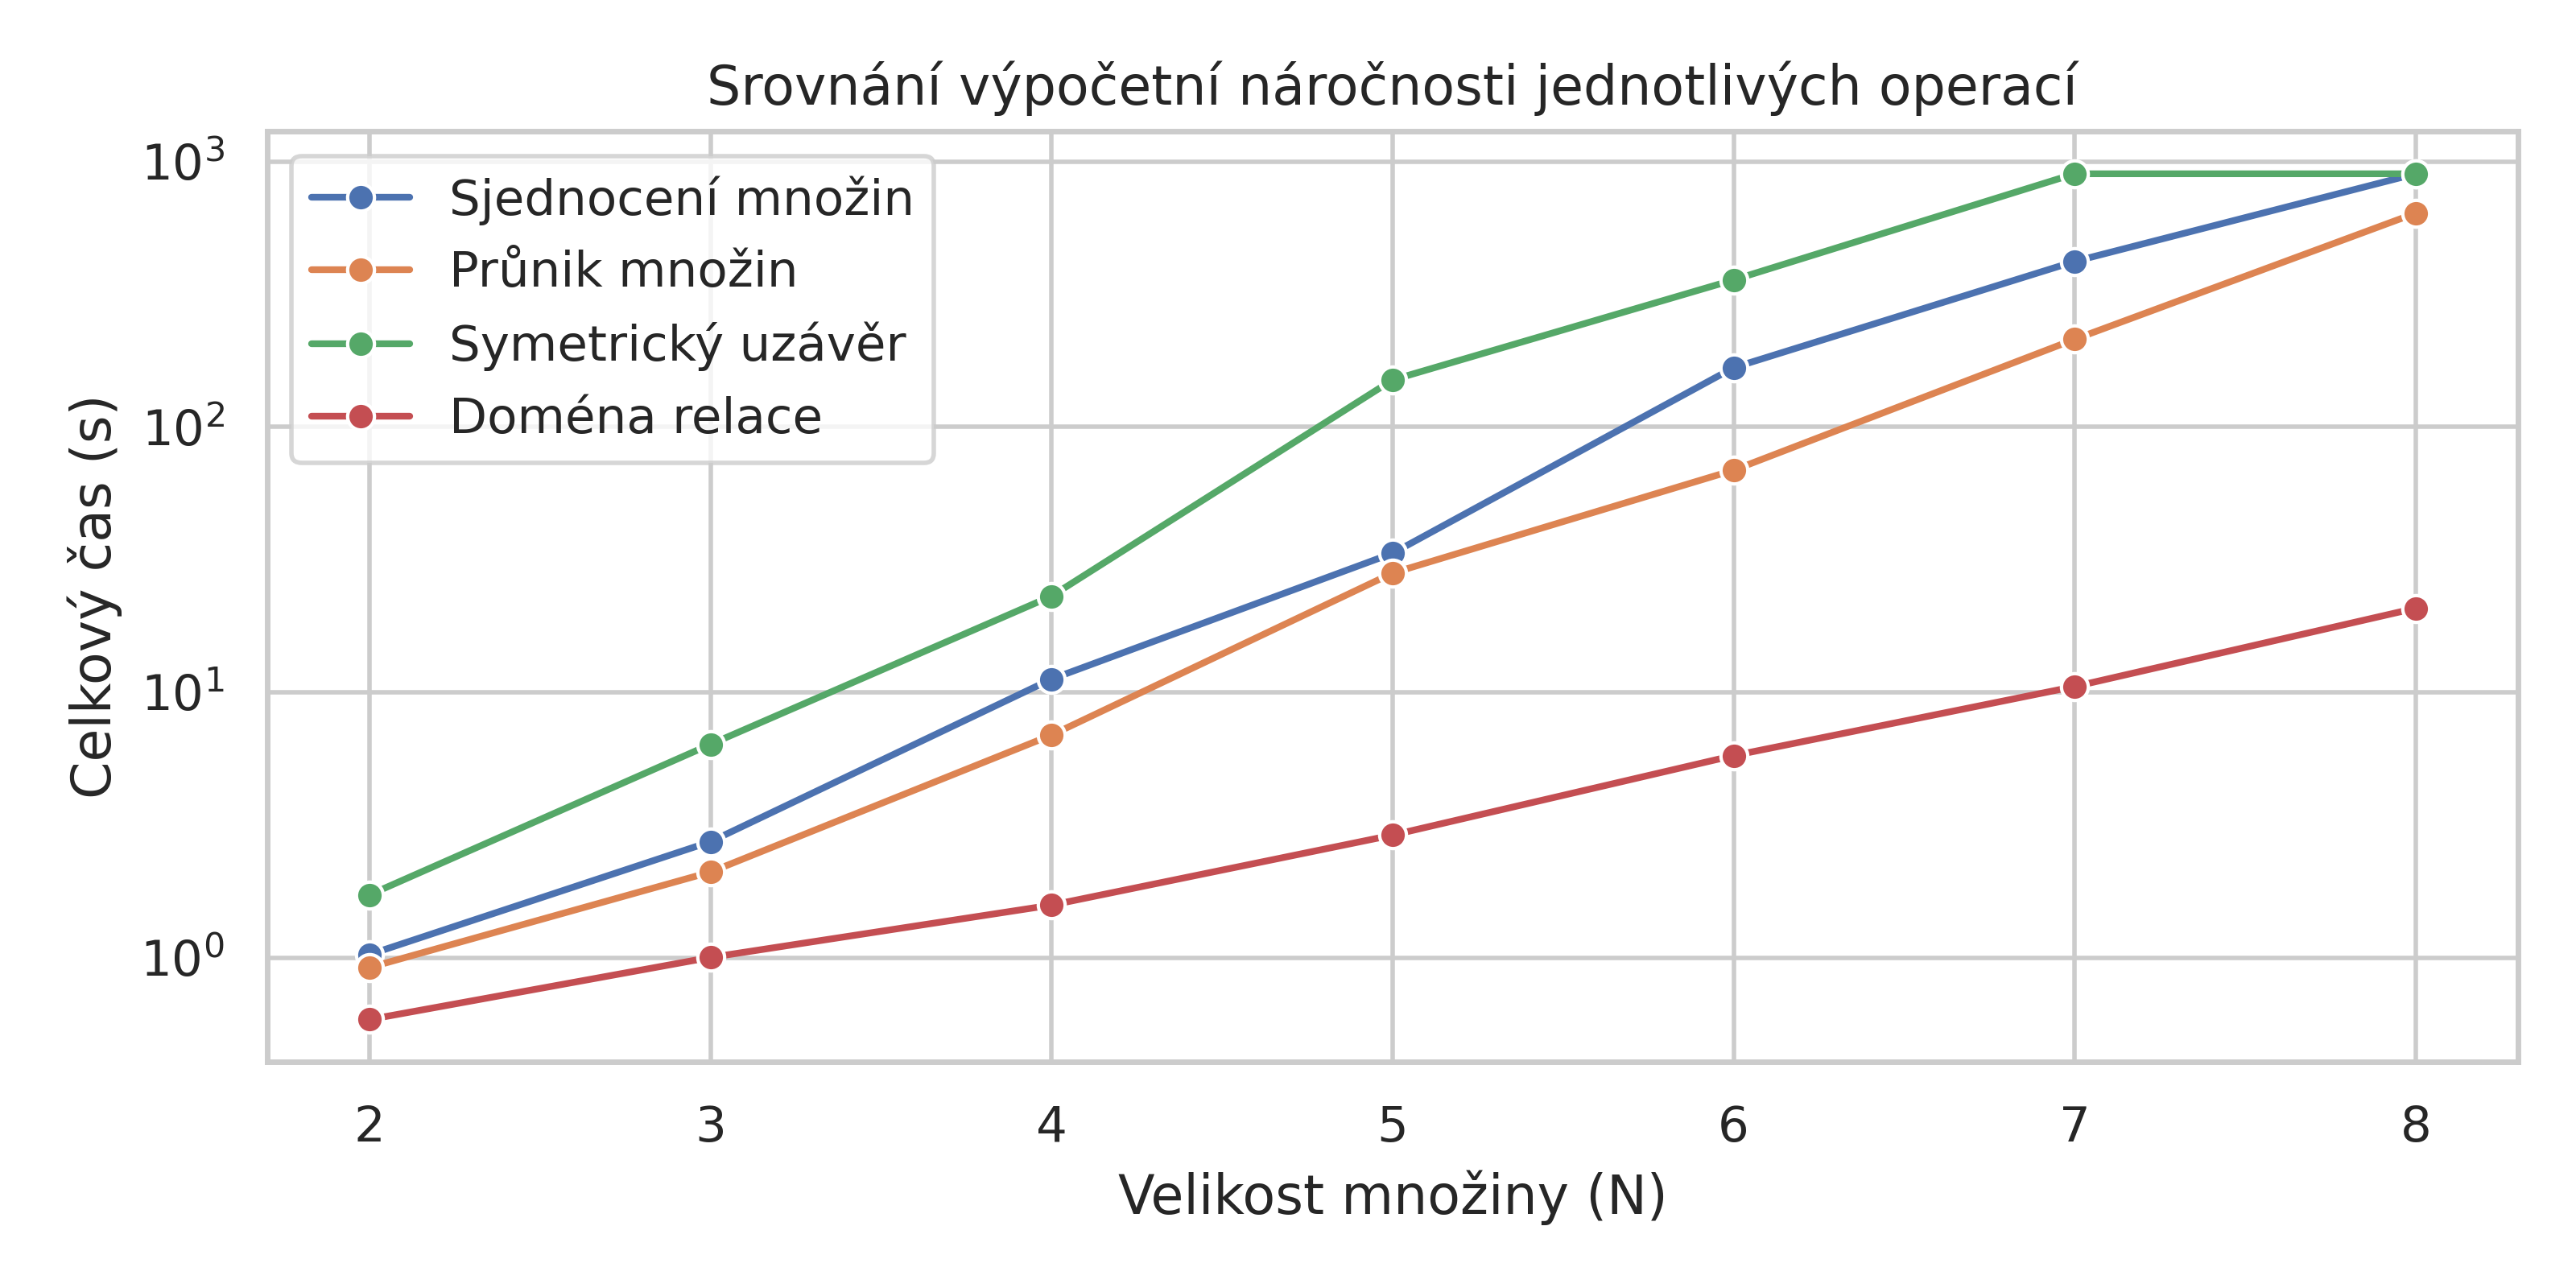
\includegraphics[width=0.8\textwidth]{img/graph_setcal_comparison.png}
    \caption{Srovnání časové náročnosti verifikace jednotlivých operací v~závislosti na velikosti vstupních dat.}
    \label{fig:IZP_AllOperations_TotalTime}
\end{figure}

Časově nejnáročnější operací byl výpočet symetrického uzávěru.
Jak je patrné z~grafu \ref{fig:IZP_AllOperations_TotalTime}, pro velikosti množin 7 a~8 verifikace dosáhla časového limitu 15 minut a~nebyla dokončena.
Důvodem je extrémní nárůst velikosti generované SAT formule.
Vztah mezi velikostí vstupu a~počtem klauzulí ve výsledné formuli pro tuto operaci ukazuje obrázek~\ref{fig:IZP_SymClosure_Clauses}.
\begin{figure}[h]
    \centering
    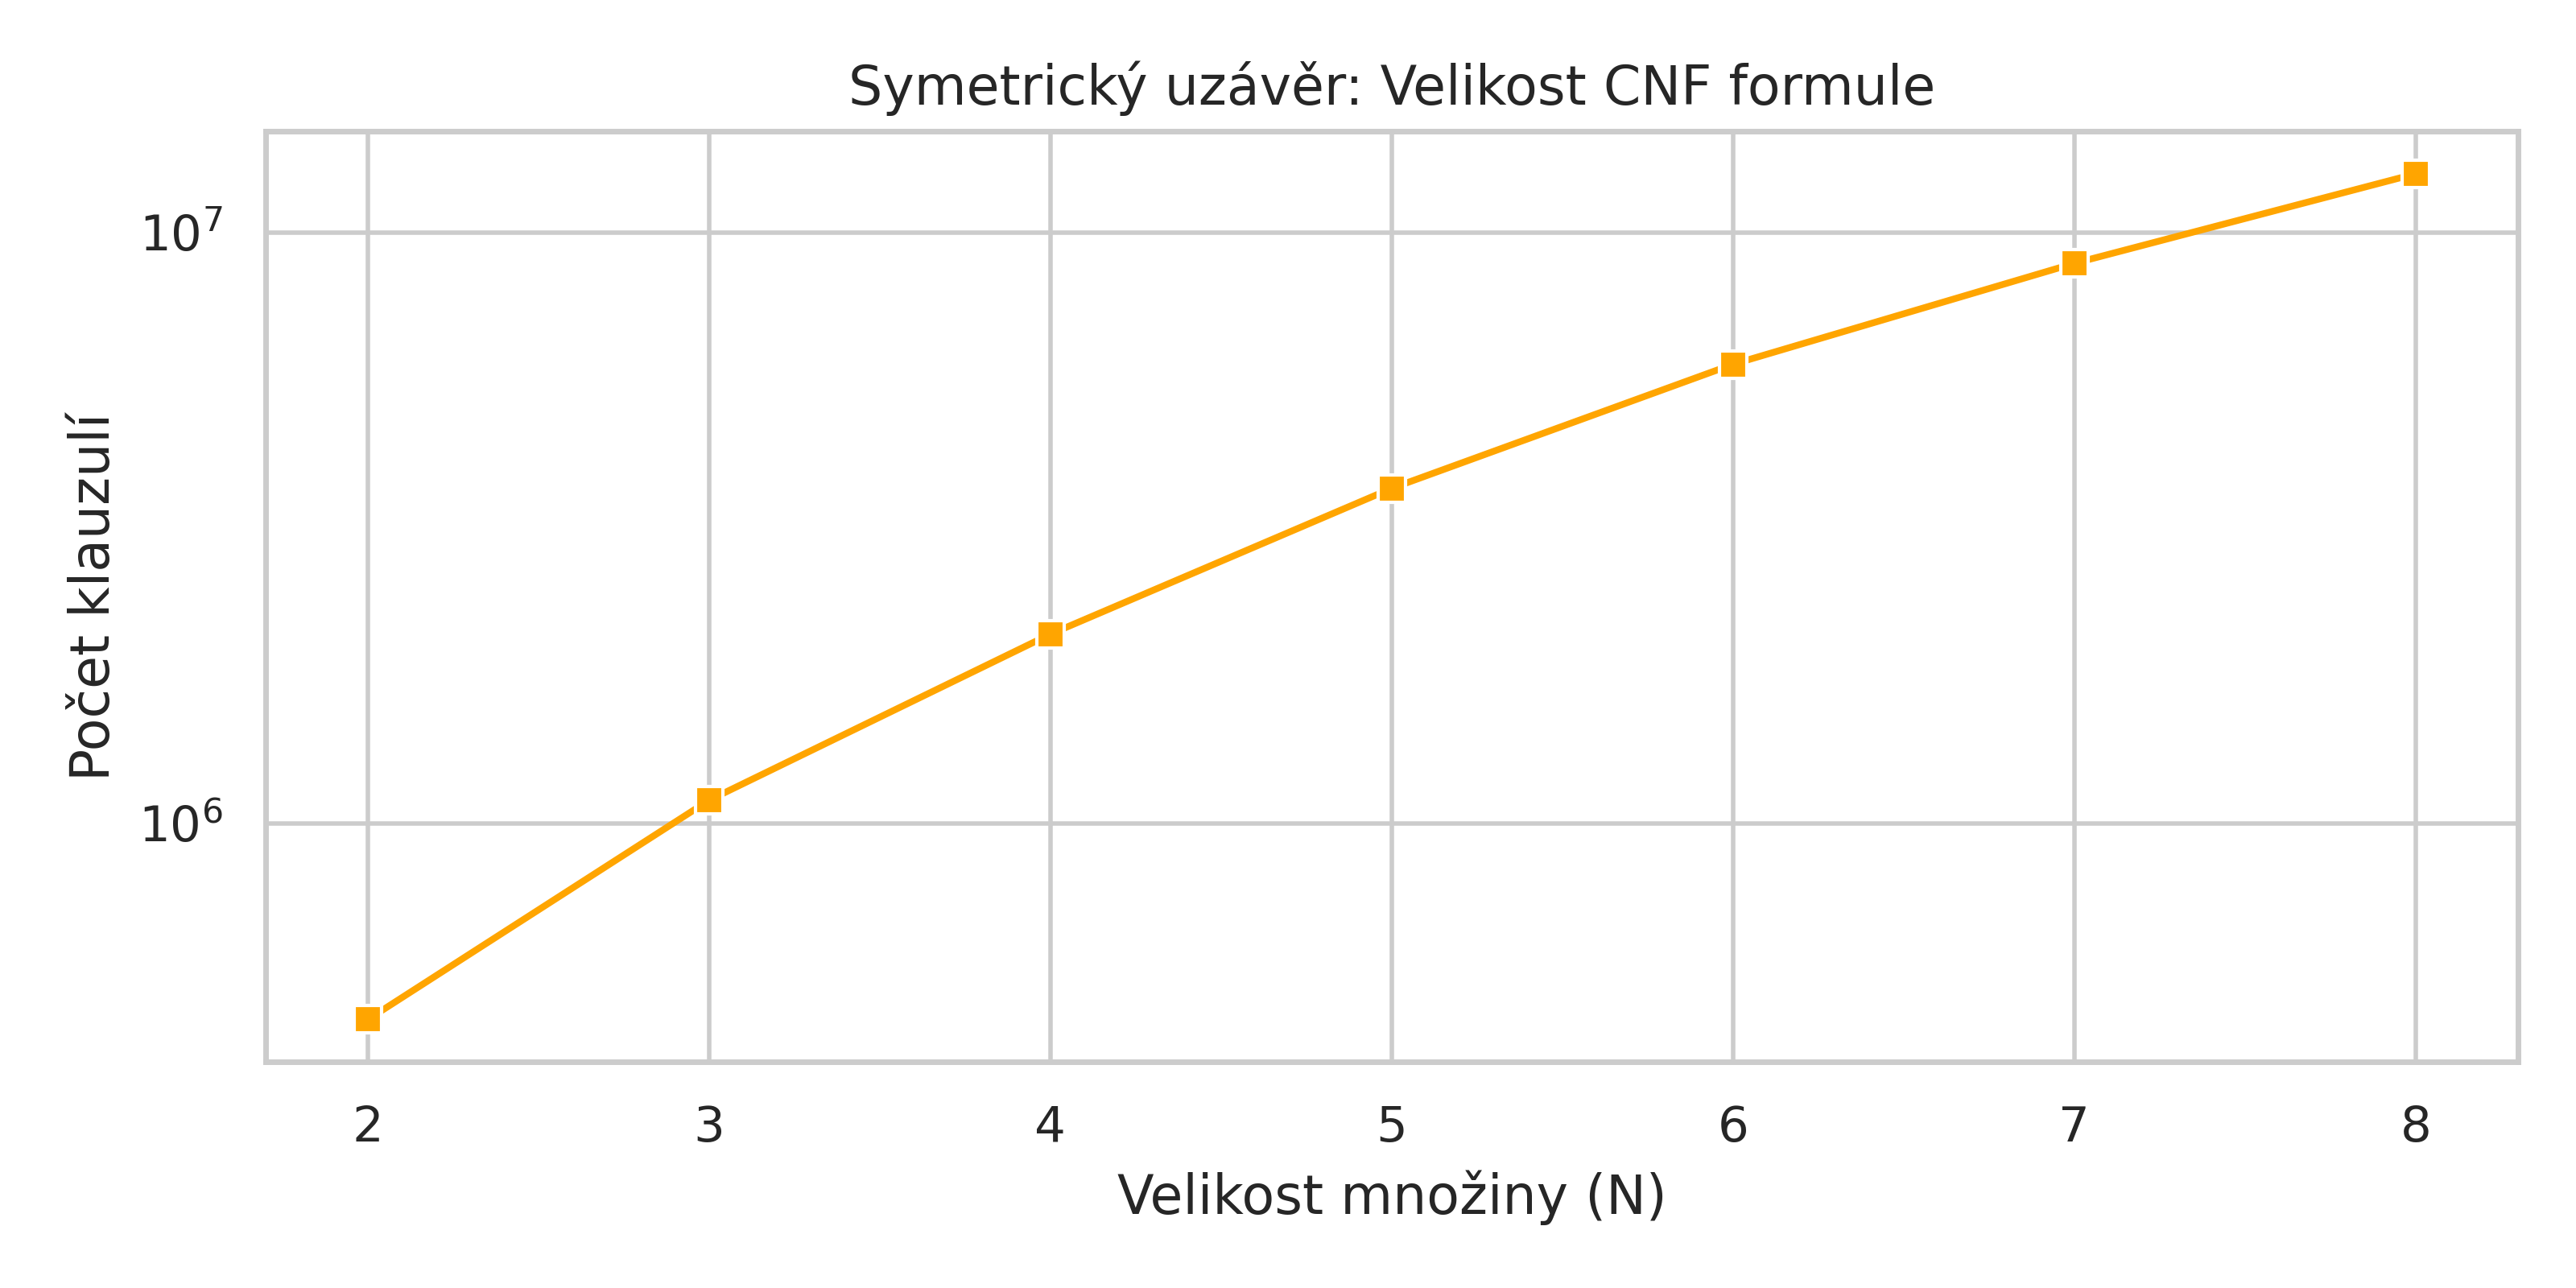
\includegraphics[width=0.8\textwidth]{img/graph_closure_sym_clauses.png} 
    \caption{Exponenciální nárůst počtu klauzulí SAT formule pro operaci symetrického uzávěru.}
    \label{fig:IZP_SymClosure_Clauses}
\end{figure}

Zatímco pro malé vstupy se pohybujeme v~řádu statisíců klauzulí, pro množinu o~velikosti 8 dosáhla výsledná formule velikosti 12 milionů klauzulí.
Takový objem dat již SAT solver nedokázal v~rozumném čase zpracovat.

Operace sjednocení a~průniku množin vykazovaly podobnou náročnost.
U~průniku byly všechny instance úspěšně verifikovány, i~když poslední instance se limitu blížila.
Sjednocení množin bylo výpočetně mírně náročnější a~verifikace největší instance o~velikosti 8 skončila vypršením časového limitu.
Velikosti formulí se zde pohybovaly od nižších stovek tisíc do jednotek milionů klauzulí.

Nejméně náročnou operací bylo hledání domény relace.
Verifikace proběhla velmi rychle, v~řádu desítek sekund i~pro největší instance.
Tomu odpovídá i~velikost formulí, kde poslední dvě instance jen lehce přesáhly jeden milion klauzulí, což je vidět na obrázku~\ref{fig:IZP_RelDomain_Clauses}.
\begin{figure}[h]
    \centering
    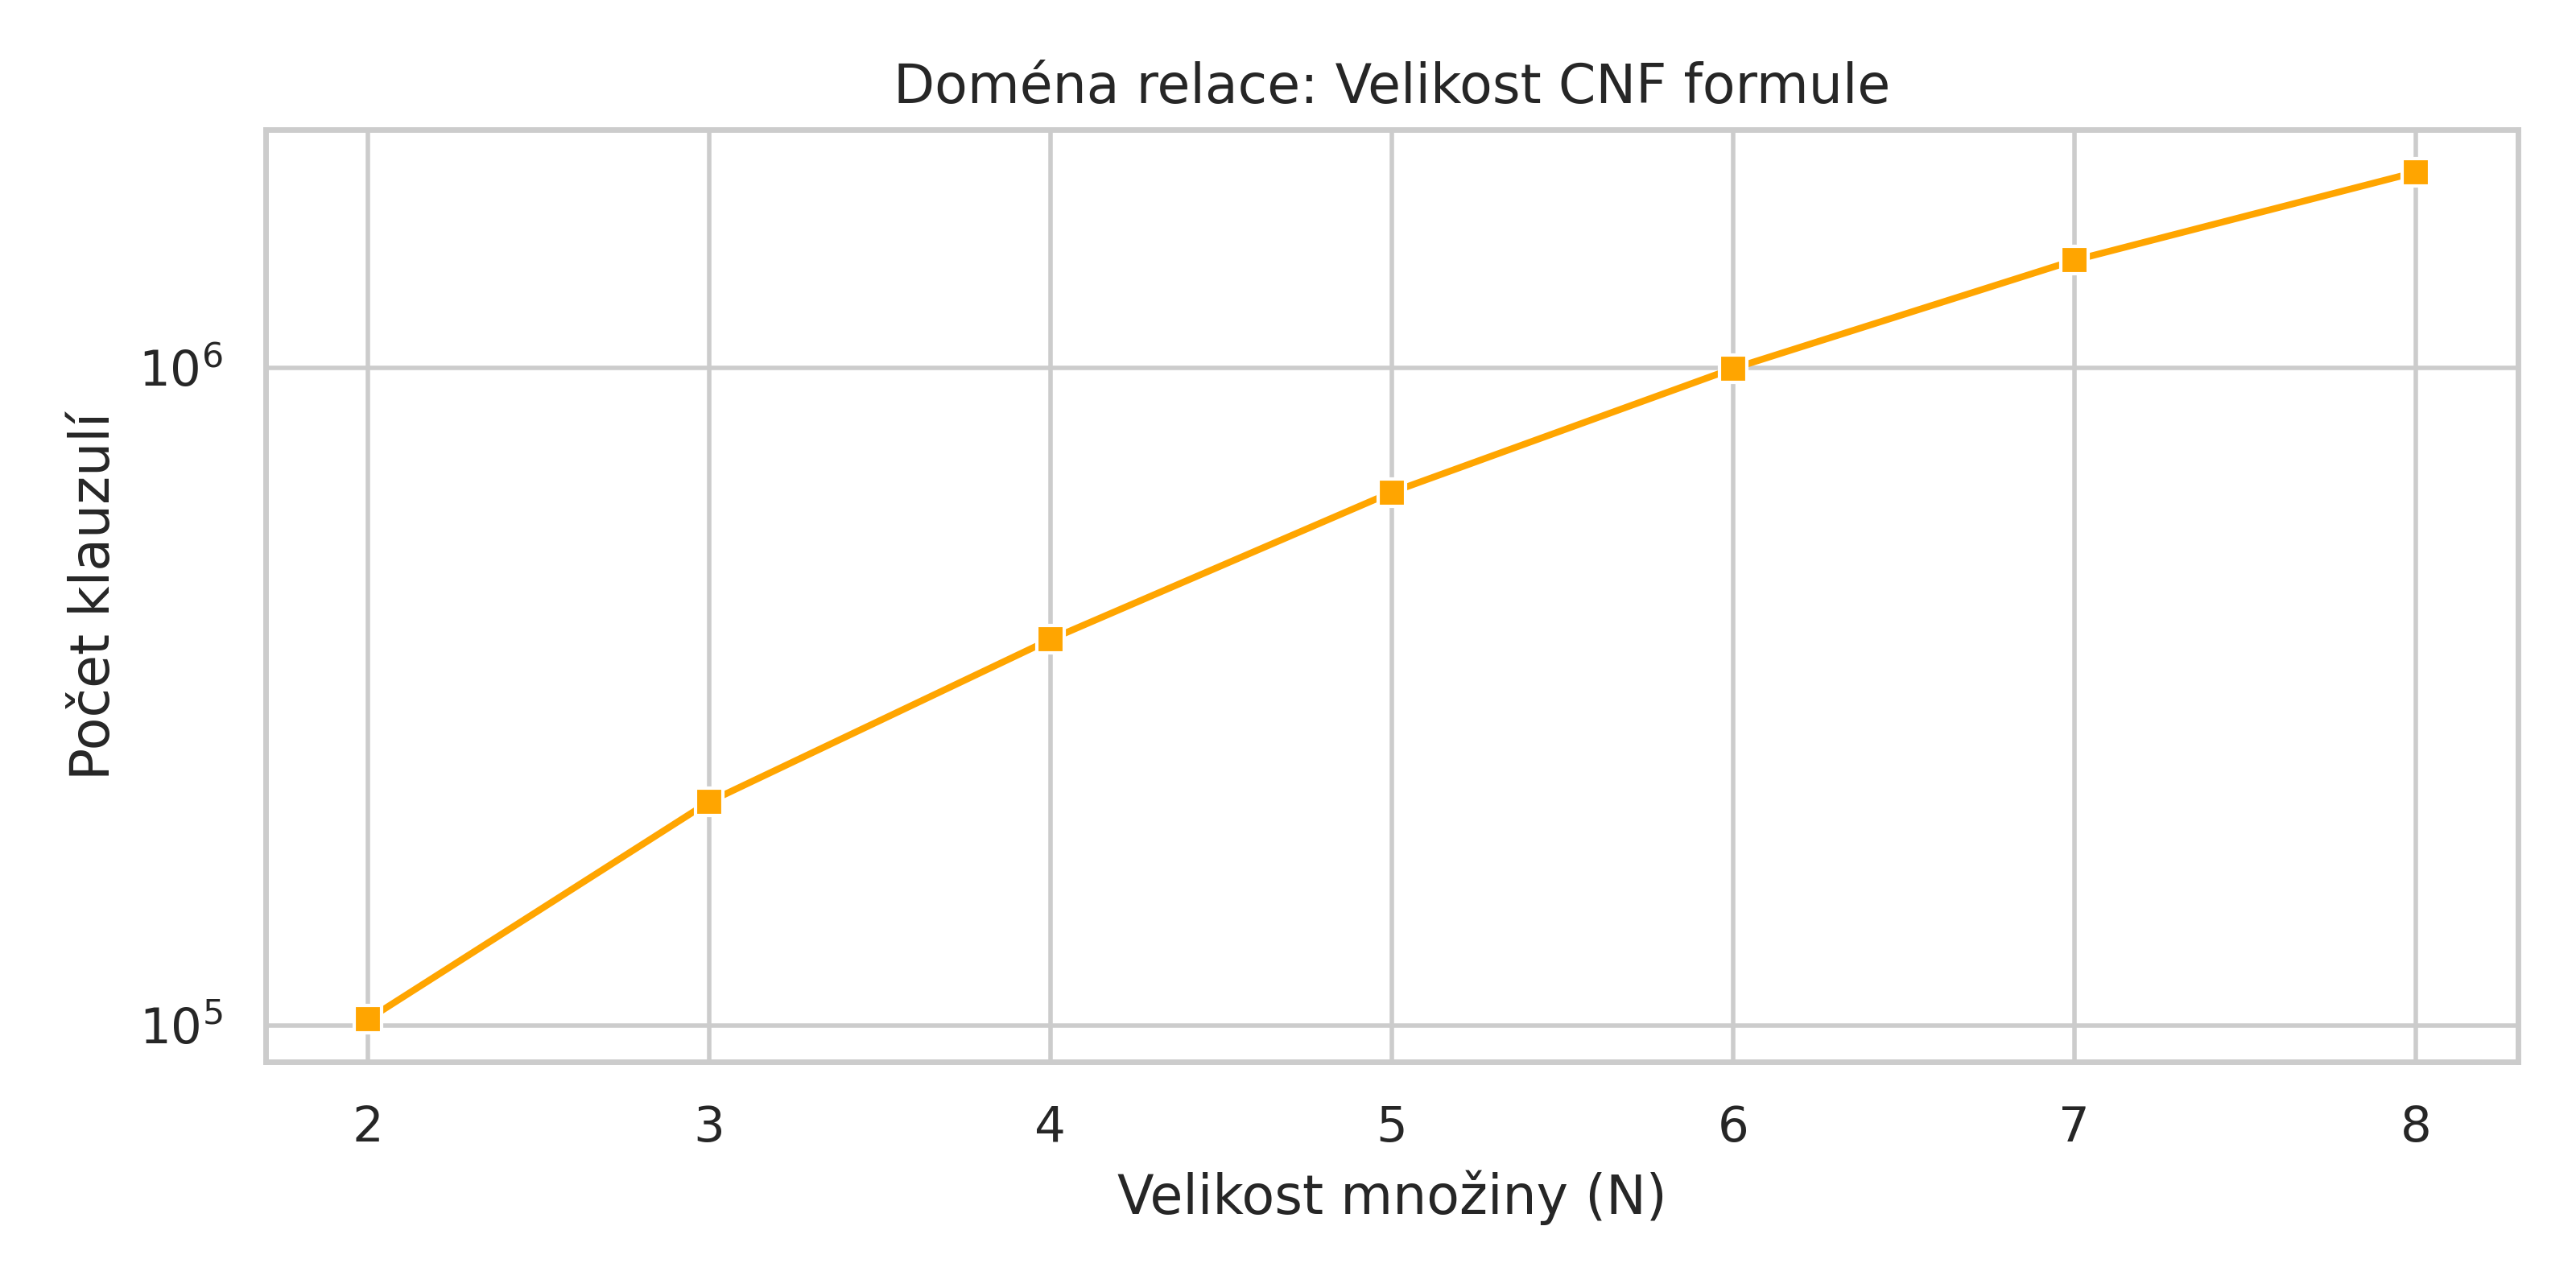
\includegraphics[width=0.8\textwidth]{img/graph_rel_domain_clauses.png}
    \caption{Exponenciální nárůst počtu klauzulí SAT formule pro operaci vyhledání domény relace.}
    \label{fig:IZP_RelDomain_Clauses}
\end{figure}
I~zde je však zřejmý exponenciální trend nárůstu stavového prostoru, ačkoliv absolutní čísla jsou řádově nižší než u~symetrického uzávěru.

\subsection{Verifikace implementace kalkulačky ovládané rotačním enkodérem}\label{sec:CBMC_Experiments_IMP}

Druhým analyzovaným projektem je firmware pro mikrokontrolér (konkrétně Kinetis K60), který provádí funkci jednoduché kalkulačky.
Je ovládána rotačním enkodérem, který má zároveň funkcionalitu tlačítka.
Logika programu je rozdělena na obsluhu hardwarových vstupů a~samotnou aplikační logiku.

Pro CBMC je největší problém závislost programu na konkrétním hardwaru, protože program přímo přistupuje ke konkrétním registrům.
Aby analýza byla možná, je možné tyto registry simulovat nedeterministickými hodnotami nebo izolovat čistě algoritmické části kódu.
V~rámci tohoto experimentu se zaměříme na druhou metodu a~budeme verifikovat ukládání nových výsledků operací do cyklického bufferu, konkrétně budeme zkoumat přístup k~tomuto poli.

\subsubsection{Analýza cyklického bufferu a detekce chyby}

Modul \texttt{result\_array.c} implementuje cyklický buffer fixní velikosti 5, do kterého se ukládají nově spočítané výsledky.
Implementace je pomocí indexu \texttt{i}, který se s~novým prvkem dekrementuje a~po dosažení indexu 0 je zresetován zpět na nejvyšší index v~bufferu.
Cílem verifikace tohoto modulu je ověření, že kód správně přistupuje do pole a~nedochází k~zápisu mimo vyhrazenou paměť.
Nicméně po spuštění CBMC byla zjištěna závažná chyba, a~to \emph{off-by-one} přístup do nealokované části paměti.

Funkce \texttt{InsertResult} implementující přidávání prvků do pole je v~programu~\ref{lst:IMP_InsertResult}.
\begin{listing}[h]
    \caption{Funkce \texttt{InsertResult} implementující vkládání nově vypočtených výsledků do cyklického pole.}
    \label{lst:IMP_InsertResult}
    \begin{minted}[
        linenos, 
        xleftmargin=1.6em, 
        fontsize=\footnotesize,
        escapeinside=@@
    ]{c}
void InsertResult(CalcData* result)
{
    static int i = PREVIOUS_RESULTS_SIZE - 1;
    newestResult = i;
    lastResults[i] = *result;
    i--;
    if (i == 0) {
        i = PREVIOUS_RESULTS_SIZE; @\label{code:IMP_InsertResult_Bug}@
    }
    return;
}
    \end{minted}
\end{listing}
Chyba je při analýze kódu zjevná.
Na řádku \ref{code:IMP_InsertResult_Bug} se po dosažení indexu 0 vrací buffer zpět na velikost pole.
Velikost pole je sice 5, ale ihned v~dalším volání této funkce je přistoupeno mimo rozsah alokovaného pole na šestou položku.
V~důsledku nízké komplexnosti programu a~malého využití zásobníku se chyba během implementace a~používání vůbec neprojevila.
Je to ale zákeřná chyba, kvůli které se mohou omylem přepsat 4 byty dat, jež mohou být kriticky důležité, především ve světě vestavěných systémů.
CBMC tuto chybu najde a~přesně řekne, kde se nachází a~jakých hodnot mají proměnné nabývat.
Výpis~\ref{lst:IMP_CBMC_Trace} ukazuje část trace vygenerované nástrojem CBMC, která demonstruje překročení hranic pole.
\begin{trace}[h]
    \caption{Výpis nástroje CBMC prokazující zápis mimo pole.}
    \label{lst:IMP_CBMC_Trace}
    \begin{lstlisting}{language=bash}
State 152 file Sources/result_array.c function InsertResult line 42 thread 0
----------------------------------------------------
  i=0 (00000000 00000000 00000000 00000000)

State 154 file Sources/result_array.c function InsertResult line 44 thread 0
----------------------------------------------------
  i=5 (00000000 00000000 00000000 00000101)

Violated property:
  file Sources/result_array.c function InsertResult line 41 thread 0
  array 'lastResults' upper bound in lastResults[(signed long int)i]    
  !((signed long int)i >= 5l)
    \end{lstlisting}
\end{trace}

Z~výpisu~\ref{lst:IMP_CBMC_Trace} je patrné, že v~okamžiku, kdy proměnná \texttt{i} dosáhne hodnoty 0 ve stavu 152, dojde k~vykonání chybné logiky pro resetování indexu.
Následně ve stavu 154 má proměnná hodnotu 5, což vede k~porušení podmínky horní meze pole.
Ve správné implementaci by na řádku~\ref{code:IMP_InsertResult_Bug} mělo být správné přiřazení \texttt{i = PREVIOUS\_RESULTS\_SIZE - 1}.

Tento experiment ukazuje sílu statické analýzy, která dokáže odhalit chyby, které se dynamickým testováním odhalují velmi obtížně.
Při testování by programátor pravděpodobně nezaznamenal žádné neobvyklé chování, ale při nasazení do produkce by chyba tohoto typu mohla způsobit pád kritického systému.

\subsubsection{Verifikace stavového automatu}
V~druhém experimentu se zaměříme na verifikaci řídicí logiky stavového automatu.
Cílem je nalézt takovou sekvenci vstupních signálů z~rotačního enkodéru, která by uvedla systém do nevalidního nebo neošetřeného stavu.
Konkrétně budeme ověřovat návratovou hodnotu funkce obsluhující stavový automat. 

Tento experiment demonstruje schopnost CBMC abstrahovat od hardwarové vrstvy.
Místo čtení hodnot z~fyzických registrů, které nejsou při statické analýze dostupné, instrumentujeme kód tak, aby vracel nedeterministické hodnoty simulující chování reálného hardwaru.
Ukázka této instrumentace je k~dispozici v~příloze~\ref{app:IMP_Instrumentation} v~programech \ref{lst:IMP_FSM_Instrumentation} a~\ref{lst:IMP_FSM_VerificationLoop}.

Korektní stavový automat může vrátit jednu z~následujících hodnot:
\begin{itemize}
    \item \texttt{ENCODER\_CW} nebo \texttt{ENCODER\_CCW} při detekci otočení po/proti směru hodinových ručiček,
    \item \texttt{ENCODERX\_BTN\_PRESSED}, kde $X \in \{1, 2\}$, při stisku tlačítka jednoho z~enkodérů,
    \item \texttt{CLEAR\_BTN} při detekci resetovacího tlačítka.
\end{itemize}
Verifikační podmínkou je, že po libovolné sekvenci interakcí musí funkce vrátit validní hodnotu z~této množiny, nebo zůstat ve stavu \texttt{IDLE}, pokud žádná interakce není zaznamenána.

Analýza byla spuštěna pro sekvence interakcí o~délce maximálně 200 kroků.
Zajímavým zjištěním tohoto experimentu je výrazný nepoměr mezi dobou předzpracování a~samotným řešením formule.
Celkový čas běhu byl přibližně 74\,s, přičemž 72\,s zabralo předzpracování a~generování formule a~pouhé 2 sekundy trvalo řešení SAT problému.
Ačkoliv vygenerovaná formule obsahovala přes 1,5 milionu klauzulí, její logická struktura byla pravděpodobně pro SAT solver triviální, což vedlo k~velmi rychlému vyřešení.

Výsledek experimentu potvrdil, že logika stavového automatu je s~vysokou pravděpodobností implementována korektně.
Vzhledem k~tomu, že zpracování jednoho fyzického otočení enkodérem trvá maximálně 4 iterace automatu a~následné interakce jsou na těch předchozích nezávislé, zvolená hloubka verifikace (200 iterací) dostatečně pokrývá stavový prostor potřebný k~odhalení případných chyb v~logice přechodů.

\section{Závěr}

Cílem této technické zprávy byla podrobná analýza nástroje CBMC, který využívá techniku \emph{bounded model checking} pro formální verifikaci programů v~jazyce C.

V~kapitole~\ref{sec:CBMC_Desc} jsme se věnovali vnitřní architektuře nástroje a~jeho formálním vlastnostem.
Popsali jsme proces předzpracování vstupního programu, jeho převod do interní reprezentace a~následné generování ekvisplnitelné SAT formule, která je poté řešena SAT solverem.

Kapitola~\ref{sec:CBMC_Demo} demonstrovala funkčnost nástroje z~praktického hlediska.
Na sadě syntetických příkladů jsme ukázali schopnost CBMC detekovat chyby, jejichž odhalení pomocí dynamického testování bývá obtížné.
Druhá část kapitoly se věnovala řadícímu algoritmu \emph{Merge sort}, na kterém jsme ilustrovali limity této techniky.
Experimenty potvrdily extrémní nárůst výpočetní náročnosti i~pro velmi malé vstupy.

V~kapitole~\ref{sec:CBMC_Experiments} jsme se zaměřili na aplikaci nástroje na reálné kódy z~vybraných univerzitních projektů.
Vzhledem k~vysoké výpočetní náročnosti jsme verifikovali pouze klíčové komponenty těchto programů.
Komplexní formální verifikace celých projektů by byla pro rozumně nastavenou hloubku rozbalení časově neproveditelná.

Tato zpráva tak poskytuje ucelený přehled o~možnostech nástroje CBMC, včetně zhodnocení jeho výhod a~omezení při verifikaci složitějších softwarových systémů.

\pagebreak

\printbibliography[title=Zdroje]

\appendix

\section{Kód řadícího algoritmu Merge sort}\label{app:merge_sort}

\begin{listing}[H]
    \caption{Kód řadícího algoritmu Merge sort analyzovaného v sekci \ref{sec:CBMC_Demo_MergeSort}.}
    \label{lst:merge_sort}
    \begin{minted}[
        linenos, 
        xleftmargin=1.6em, 
        fontsize=\footnotesize,
        escapeinside=@@
    ]{c}
#define SIZE 5

int nondet_int();

void Merge(int arr[], int left, int mid, int right)
{
    int i, j, k;
    int left_subarray_size = mid - left + 1;
    int right_subarray_size = right - mid;
    int left_subarray[left_subarray_size], right_subarray[right_subarray_size];

    // Copy data to temp arrays L[] and R[]
    for (i = 0; i < left_subarray_size; i++)
        left_subarray[i] = arr[left + i];
    for (j = 0; j < right_subarray_size; j++)
        right_subarray[j] = arr[mid + 1 + j];

    i = 0;
    j = 0;
    k = left;
    // Merge back into arr[l..r]
    while (i < left_subarray_size && j < right_subarray_size) {
        if (left_subarray[i] <= right_subarray[j]) { @\label{code:merge_sort_bug_condition}@
            arr[k] = left_subarray[i];
            i++;
        }
        else {
            arr[k] = right_subarray[j];
            j++;
        }
        k++;
    }

    // Copy the remaining elements of L[], if any are left
    while (i < left_subarray_size) { @\label{code:copy_remaining_start}@
        arr[k] = left_subarray[i];
        i++;
        k++;
    }
    // Copy the remaining elements of R[], if any are left
    while (j < right_subarray_size) { 
        arr[k] = right_subarray[j];
        j++;
        k++;
    } @\label{code:copy_remaining_end}@
}
    \end{minted}
\end{listing}

\pagebreak

\begin{listing}[H]
    \ContinuedFloat
    \caption[]{Kód řadícího algoritmu Merge sort -- pokračování}
    \begin{minted}[
        linenos,
        xleftmargin=1.6em,
        fontsize=\footnotesize,
        firstnumber=47
    ]{c}
void merge_sort(int arr[], int left, int right)
{
    if (left < right) {
        int mid = left + (right - left) / 2;

        merge_sort(arr, left, mid);
        merge_sort(arr, mid + 1, right);

        Merge(arr, left, mid, right);
    }
}

int main()
{
    int arr[SIZE];

    for (int i = 0; i < SIZE; i++) {
        arr[i] = nondet_int();
    }

    merge_sort(arr, 0, SIZE - 1);

    for (int i = 0; i < SIZE - 1; i++) {
        assert(arr[i] <= arr[i + 1]);
    }

    return 0;
}
    \end{minted}
\end{listing}

\pagebreak

\section{Instrumentace kódu pro verifikaci stavového automatu}\label{app:IMP_Instrumentation}

\begin{listing}[h]
    \caption{Instrumentovaná hlavička souboru \texttt{fsm.c} implementující logiku stavového automatu. Jsou vytvořeny falešné registry, které jsou poté v~rámci hlavní smyčky naplněny nedeterministickými hodnotami na začátku každé iterace.}
    \label{lst:IMP_FSM_Instrumentation}
    \begin{minted}[
        linenos, 
        xleftmargin=1.6em, 
        fontsize=\footnotesize,
        escapeinside=@@
    ]{c}
#ifdef CBMC_VERIFICATION
// mock hardware pro cbmc
#include <stdint.h>
int nondet_int();

typedef struct
{
    uint32_t PDIR;
} GPIO_Type;

GPIO_Type mock_pta;
GPIO_Type mock_pte;

GPIO_Type* PTA = &mock_pta;
GPIO_Type* PTE = &mock_pte;

#    define FSM_LOOP_LIMIT 200
#else
// realny hardware
#    include "MK60D10.h"
#endif
    \end{minted}
\end{listing}

\begin{listing}[H]
    \caption{Část původního kódu implementující stavový automat využívající \uv{nové} registry definované pro analýzu. Navíc je uveden limit pro počet iterací cyklu, který reprezentuje maximální délku posloupnosti jednotlivých akcí, které uživatel provede s~rotačním enkodérem.}
    \label{lst:IMP_FSM_VerificationLoop}
    \begin{minted}[
        linenos, 
        xleftmargin=1.6em, 
        fontsize=\footnotesize,
        escapeinside=@@
    ]{c}
#ifdef CBMC_VERIFICATION
// Verifikace -- omezeny pocet kroku
for (int iter = 0; iter < FSM_LOOP_LIMIT; iter++) {
    PTA->PDIR = nondet_int();
    PTE->PDIR = nondet_int();
#else
// Puvodni nekonecna smycka pro mikrokontroler
while (1) {
#endif
    a = !(PTA->PDIR & (1 << pin_a));
    b = !(PTA->PDIR & (1 << pin_b));
    btn = !(PTA->PDIR & (1 << pin_btn1));
    clr_btn = !(PTE->PDIR & (1 << pin_clr_btn));
    \end{minted}
\end{listing}

\end{document}
